\newcommand{\sigtextable}{Standard errors (reported in parentheses) are clustered at the bank level. We use *,**, and *** to denote statistical significance at the 10\%, 5\%, and 1\% levels, respectively.}

\clearpage
\begin{figure}
    \centering
    \adddescription{
    \small
This figure presents the evolution of the U.S. banking system. Panel A shows the total number of banks (blue line, left axis) and the total number of bank offices (orange line, right axis). Panel B displays the annual number of branch openings (blue line) and closures (orange line) from 2001 to 2023.
    }
    Panel A: Total Number of Banks and Branches
    \includegraphics[width=0.7\textwidth]{resources/figures/old/bank_branch_line_plot.jpg}\\
    \vspace{1cm}
    Panel B:  Branch Openings and Closures
    \includegraphics[width=0.7\textwidth]{resources/figures/JF figures/gross_open_closed.jpg}
    \caption{Change in Banks and Branches}
    \label{fig:no_of_banks_branches}
\end{figure}



\clearpage
\begin{figure}
    \centering
    \adddescription{
    \small
This figure presents the annual percentage of branches closed and opened by large banks ($\geq$ \$100 billion in assets, blue line) and small banks ($<$\$100 billion in assets, orange line) from 2001 to 2023. Panel A shows the percentage of branches closed each year. Panel B shows the percentage of new branches opened each year.
    }
    Panel A: Percent of Branch Closures
    \includegraphics[width=0.7\textwidth]{resources/figures/JF figures/closed_pct_by_size.jpg}\\
    \vspace{1cm}
    Panel B:  Percent of Branch Openings
    \includegraphics[width=0.7\textwidth]{resources/figures/JF figures/open_pct_by_size.jpg}\\
    \caption{Percent of Openings and Closures}
    \label{fig:pct_branches_closed}
\end{figure}


\clearpage
\begin{table}[]
    \centering
    \adddescription{
    \small
This table presents summary statistics for the bank-level samples during three interest rate cycles, separately for large banks ($\geq$ \$100 billion in assets) and small banks ($<$ \$100 billion in assets). Panels A, B, and C correspond to the Late (2022-2023), Mid (2016-2019), and Early (2004-2006) cycles, respectively. For each group, the table reports the mean, standard deviation (SD), and selected percentiles for variables.
    }
    \vspace{0.5cm}
    {\small Panel A: Late Cycle (2022-2023)}
    \resizebox{0.8\textwidth}{!}{
       \begin{tabular}{lrrrrrrrr}
  \hline

& \multicolumn{4}{c}{Large Banks (Obs = 27)} & \multicolumn{4}{c}{Small Banks (Obs = 4,296)} \\
\cmidrule(l){2-5} \cmidrule(l){6-9}
Variable & Mean & SD & P10 & P90 & Mean & SD & P10 & P90 \\ 
  \hline
Age & 37.73 & 3.25 & 34.21 & 41.66 & 40.72 & 4.31 & 35.56 & 45.71 \\ 
  College educated fraction & 0.57 & 0.15 & 0.41 & 0.80 & 0.29 & 0.14 & 0.16 & 0.49 \\ 
  Deposit-weighted Pop. density & 0.52 & 0.14 & 0.36 & 0.69 & 0.15 & 0.21 & 0.01 & 0.57 \\ 
  Deposit beta & 0.32 & 0.14 & 0.18 & 0.55 & 0.18 & 0.12 & 0.04 & 0.35 \\ 
  Family income (000) & 88.81 & 39.06 & 59.00 & 117.00 & 58.28 & 18.45 & 39.00 & 80.00 \\ 
  Frac. deposits in sophisticated zipcodes & 0.82 & 0.17 & 0.56 & 1.00 & 0.46 & 0.41 & 0.00 & 1.00 \\ 
  HHI & 0.23 & 0.12 & 0.13 & 0.29 & 0.24 & 0.13 & 0.11 & 0.40 \\ 
  Stock market participation frac & 0.32 & 0.12 & 0.19 & 0.45 & 0.20 & 0.08 & 0.10 & 0.29 \\ 
   \hline
\end{tabular}
        }
    \\
    \vspace{0.5cm}
{\small Panel B: Mid Cycle (2016-2019)}

    \resizebox{0.8\textwidth}{!}{
   \begin{tabular}{lrrrrrrrr}
  \hline
  & \multicolumn{4}{c}{Large Banks (Obs = 38)} & \multicolumn{4}{c}{Small Banks (Obs = 4,872)} \\
\cmidrule(l){2-5} \cmidrule(l){6-9}
Variable & Mean & SD & P10 & P90 & Mean & SD & P10 & P90 \\ 
  \hline
Age & 37.37 & 3.30 & 33.22 & 40.73 & 40.73 & 4.34 & 35.57 & 45.73 \\ 
  College educated fraction & 0.55 & 0.16 & 0.38 & 0.77 & 0.30 & 0.15 & 0.16 & 0.51 \\ 
  Deposit-weighted Pop. density & 0.51 & 0.15 & 0.28 & 0.69 & 0.15 & 0.21 & 0.01 & 0.58 \\ 
  Deposit beta & 0.24 & 0.10 & 0.13 & 0.38 & 0.17 & 0.12 & 0.03 & 0.34 \\ 
  Family income (000) & 89.10 & 36.37 & 58.70 & 117.20 & 58.97 & 19.02 & 40.00 & 83.00 \\ 
  Frac. deposits in sophisticated zipcodes & 0.77 & 0.27 & 0.46 & 1.00 & 0.46 & 0.41 & 0.00 & 1.00 \\ 
  HHI & 0.24 & 0.17 & 0.14 & 0.30 & 0.23 & 0.13 & 0.11 & 0.38 \\ 
  Stock market participation frac & 0.30 & 0.12 & 0.16 & 0.45 & 0.20 & 0.09 & 0.10 & 0.30 \\ 
   \hline
\end{tabular}
    }

\vspace{0.5cm}
{\small Panel C: Early Cycle (2004-2006)}

    \resizebox{0.8\textwidth}{!}{
   \begin{tabular}{lrrrrrrrr}
  \hline
    & \multicolumn{4}{c}{Large Banks (Obs = 32)} & \multicolumn{4}{c}{Small Banks (Obs = 5,515)} \\
\cmidrule(l){2-5} \cmidrule(l){6-9}
Variable & Mean & SD & P10 & P90 & Mean & SD & P10 & P90 \\ 
  \hline
Age & 37.65 & 2.36 & 34.30 & 39.54 & 39.89 & 4.31 & 34.76 & 45.29 \\ 
  College educated fraction & 0.51 & 0.13 & 0.38 & 0.72 & 0.27 & 0.13 & 0.14 & 0.45 \\ 
  Deposit-weighted Pop. density & 0.48 & 0.12 & 0.30 & 0.65 & 0.13 & 0.19 & 0.01 & 0.51 \\ 
  Deposit beta & 0.29 & 0.12 & 0.12 & 0.41 & 0.23 & 0.11 & 0.10 & 0.38 \\ 
  Family income (000) & 71.03 & 23.75 & 48.00 & 90.70 & 50.36 & 15.34 & 35.00 & 70.00 \\ 
  Frac. deposits in sophisticated zipcodes & 0.76 & 0.20 & 0.54 & 1.00 & 0.44 & 0.42 & 0.00 & 1.00 \\ 
  HHI & 0.22 & 0.13 & 0.12 & 0.32 & 0.24 & 0.14 & 0.11 & 0.40 \\ 
  Stock market participation frac & 0.29 & 0.10 & 0.22 & 0.39 & 0.20 & 0.08 & 0.11 & 0.29 \\ 
   \hline
\end{tabular}
}
\caption{Descriptive Statistics - Bank Level}
\label{tab:bank_desc_stats}
\end{table}


\clearpage
\begin{figure}
    \centering
    \adddescription{
    \small
This figure presents density plots of  deposit beta values across three interest rate cycles: Early (2004-2006), Mid (2016-2019), and Late (2022-2023). Panel A displays bank-level beta distributions, while Panel B displays predicted branch-level beta distributions. In both panels, small banks (assets $<$ \$100 billion) are shown in orange, and large banks (assets $\geq$ \$100 billion) are shown in blue. Each subplot represents the distribution of beta values during the indicated interest rate cycle.
    }
     Panel A: Bank-Level\\
 
    \includegraphics[width=0.8\textwidth]{resources/figures/beta_density_bank.jpg}
        \vspace{1.5cm}\\
    Panel B: Branch-Level\\
     \vspace{0.5cm}
    \includegraphics[width=0.8\textwidth]{resources/figures/beta_density_branch.jpg}
    \caption{Deposit Beta Distribution}
    \label{fig:df_density}
\end{figure}



\begin{table}[]
    \centering
    \adddescription{
    \small
This table presents regression estimates of deposit beta from Equation (2) across three interest rate cycles: Early (2004-2006), Mid (2016-2019), and Late (2022-2023). Columns 1–3 report specifications that include individual demographic variables with other controls. Columns 4–6 report a parsimonious specification that replaces the individual demographic variables with the fraction of deposits in sophisticated zip codes, defined as zip codes with above-median levels of both education and stock market participation. The dependent variable is the deposit beta.   *, **, and *** denote statistical significance at the 10\%, 5\%, and 1\% levels, respectively.    }

    \resizebox{\textwidth}{!}{
\begin{tabular}{@{\extracolsep{5pt}}lcccccc} 
\\[-1.8ex]\hline 
\hline \\[-1.8ex] 
 & \multicolumn{6}{c}{Deposit Beta} \\ 
\cline{2-7} 
 & Early Cyc. & Mid Cyc. & Late Cyc. & Early Cyc. & Mid Cyc. & Late Cyc.\\ 
\\[-1.8ex] & (1) & (2) & (3) & (4) & (5) & (6)\\ 
\hline \\[-1.8ex] 
  College frac                               & 0.4026$^{***}$  & 0.3353$^{***}$  & 0.5624$^{***}$  &                 &                 &   \\   
                                              & (0.0725)        & (0.0600)        & (0.1044)        &                 &                 &   \\   
   Stock market frac                          & 0.0863          & 0.1987$^{**}$   & 0.1409          &                 &                 &   \\   
                                              & (0.1004)        & (0.0812)        & (0.1435)        &                 &                 &   \\   
   Frac of deposits in sophisticated zipcodes &                 &                 &                 & 0.0763$^{***}$  & 0.0659$^{***}$  & 0.1039$^{***}$\\   
                                              &                 &                 &                 & (0.0138)        & (0.0123)        & (0.0208)\\   
   Age Q1-Q2                                  & 0.0068          & -0.0002         & 0.0015          & 0.0028          & -0.0016         & -0.0031\\   
                                              & (0.0129)        & (0.0107)        & (0.0181)        & (0.0127)        & (0.0105)        & (0.0177)\\   
   Age Q2-Q3                                  & -0.0204         & -0.0038         & 0.0097          & -0.0234$^{*}$   & -0.0021         & 0.0064\\   
                                              & (0.0149)        & (0.0123)        & (0.0210)        & (0.0141)        & (0.0118)        & (0.0199)\\   
   Age $>$Q3                                    & -0.0070         & -0.0641$^{***}$ & -0.0817$^{***}$ & -0.0094         & -0.0556$^{***}$ & -0.0796$^{***}$\\   
                                              & (0.0184)        & (0.0171)        & (0.0292)        & (0.0173)        & (0.0163)        & (0.0278)\\   
   log(Income)                                & -0.1278$^{***}$ & -0.0926$^{***}$ & -0.1295$^{***}$ & -0.0832$^{***}$ & -0.0186         & -0.0436\\   
                                              & (0.0267)        & (0.0234)        & (0.0395)        & (0.0233)        & (0.0201)        & (0.0338)\\   
   County deposit HHI                         & -0.1294$^{***}$ & -0.0578$^{*}$   & -0.1440$^{***}$ & -0.1309$^{***}$ & -0.0493         & -0.1428$^{**}$\\   
                                              & (0.0371)        & (0.0326)        & (0.0554)        & (0.0370)        & (0.0328)        & (0.0556)\\   
   log(Assets)                                & 0.0059          & 0.0158$^{***}$  & 0.0614$^{***}$  & 0.0077$^{*}$    & 0.0179$^{***}$  & 0.0645$^{***}$\\   
                                              & (0.0043)        & (0.0033)        & (0.0053)        & (0.0043)        & (0.0033)        & (0.0053)\\   
   Population density                         & 0.0394          & 0.0921$^{***}$  & 0.2802$^{***}$  & 0.1364$^{***}$  & 0.1806$^{***}$  & 0.4203$^{***}$\\   
                                              & (0.0355)        & (0.0285)        & (0.0484)        & (0.0313)        & (0.0248)        & (0.0422)\\   
   Transaction Accounts/Assets                & -0.5629$^{***}$ & -0.3281$^{***}$ & -0.2854$^{***}$ & -0.5650$^{***}$ & -0.3274$^{***}$ & -0.2935$^{***}$\\   
                                              & (0.0720)        & (0.0484)        & (0.0677)        & (0.0721)        & (0.0486)        & (0.0678)\\   
   Uninsured Deposits/Deposits                & 0.7734$^{***}$  & -0.0529$^{*}$   & 0.3780$^{***}$  & 0.8114$^{***}$  & -0.0253         & 0.4153$^{***}$\\   
                                              & (0.0364)        & (0.0299)        & (0.0512)        & (0.0356)        & (0.0298)        & (0.0511)\\   
  Constant                                   & 1.773$^{***}$   & 1.175$^{***}$   & 1.059$^{**}$    & 1.336$^{***}$   & 0.4230$^{*}$    & 0.1917\\   
  & (0.2844)        & (0.2505)        & (0.4218)        & (0.2546)        & (0.2190)        & (0.3681)\\   
    \\
   Observations                               & 5,539           & 4,906           & 4,405           & 5,539           & 4,906           & 4,405\\  
   R$^2$                                      & 0.17833         & 0.09642         & 0.20750         & 0.17544         & 0.08855         & 0.20282\\  
   % Adjusted R$^2$                             & 0.17670         & 0.09439         & 0.20551         & 0.17395         & 0.08669         & 0.20101\\ 
\hline 
\hline \\[-1.8ex] 
\textit{Note:}  & \multicolumn{6}{r}{$^{*}$p$<$0.1; $^{**}$p$<$0.05; $^{***}$p$<$0.01} \\ 
\end{tabular} 
    }
    \caption{Bank-Level Deposit Beta}
    \label{tab:deposit_beta_reg}
\end{table}











\clearpage
\begin{figure}
    \centering
    \adddescription{
    \small
This figure presents scatter plots comparing deposit beta between pairs of interest rate cycles. The interest rate cycles are: Early (2004-2006), Mid (2016-2019), and Late (2022-2023).  Panels A and B display branch-level observations; Panels C and D display bank-level observations. Each point represents a small bank (assets $<$ \$100 billion, orange) or a large bank (assets $\geq$ \$100 billion, blue). The x-axis reports beta in the earlier cycle, and the y-axis reports beta in the later cycle. The dashed line denotes the 45-degree reference line. The solid line represents the fitted relationship from a linear regression.   }
            \begin{subfigure}[b]{0.45\textwidth}
        \centering
        \caption*{Panel A: Bank-Level Early vs Mid Cycles}
        \includegraphics[width=\textwidth]{resources/figures/df_scatter_bank_early_mid.jpg}
        
    \end{subfigure}
    \hfill
    \begin{subfigure}[b]{0.45\textwidth}
        \centering
                \caption*{Panel B: Bank-Level Mid vs Late Cycles}
        \includegraphics[width=\textwidth]{resources/figures/df_scatter_bank_mid_late.jpg}
            \end{subfigure}

            
      \vspace{0.5cm}

    
            \begin{subfigure}[b]{0.45\textwidth}
        \centering
        \caption*{Panel C: Branch-Level  Early vs Mid Cycles}
        \includegraphics[width=\textwidth]{resources/figures/df_scatter_branch_early_mid.jpg}
        
    \end{subfigure}
    \hfill
    \begin{subfigure}[b]{0.45\textwidth}
        \centering
        \caption*{Panel D: Branch-Level Mid vs Late Cycles}
        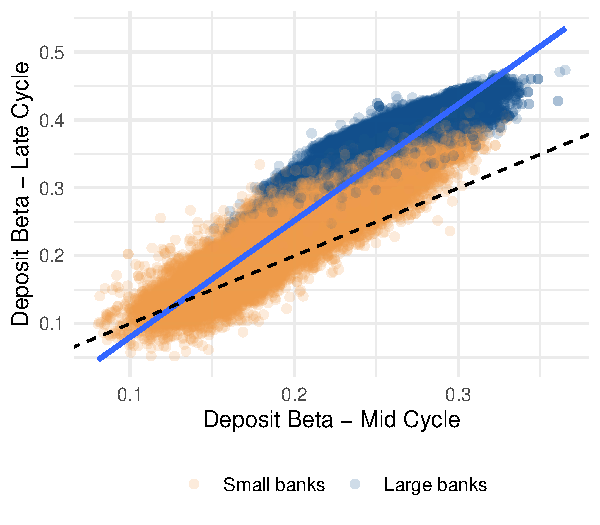
\includegraphics[width=\textwidth]{resources/figures/df_scatter_branch_mid_late.jpg}
            \end{subfigure}


    \caption{Deposit Beta Correlations Across Cycles}
    \label{fig:df_scatter}
\end{figure}


\clearpage
\begin{table}[]
    \centering
    \adddescription{
\small
This table reports regression estimates from Equation (3), examining branch usage and customer travel distance to branches. Results are shown separately for large banks ($\geq$\$100 billion in assets) and small banks ($<$\$100 billion in assets). Panel A presents estimates from a parsimonious model using a single indicator for sophisticated zip codes. Panel B reports estimates using separate demographic variables, including age quartiles, income, education, and stock market participation. Columns 1–2 report regressions where the dependent variable is branch usage, defined as the percentage drop in visits from 2019 to 2021 for each branch. Columns 3–4 use the mean distance (in kilometers) that customers traveled to visit the branch in 2019 as the dependent variable.  *, **, and *** denote significance at the 10\%, 5\%, and 1\% levels, respectively.

    }
\vspace{0.5cm}
{\small Panel A}\\
    \resizebox{0.5\textwidth}{!}{
\begin{tabular}{@{\extracolsep{5pt}}lcccc} 
\\[-1.8ex]\hline 
\hline \\[-1.8ex] 
%  & \multicolumn{4}{c}{\textit{Dependent variable:}} \\ 
% \cline{2-5} 
 & \multicolumn{2}{c}{Drop in visits} & \multicolumn{2}{c}{log(distance km)} \\ 
 \\[-1.8ex] & Large banks & Small banks & Large banks & Small banks\\ 
\\[-1.8ex] & (1) & (2) & (3) & (4)\\ 
\hline \\[-1.8ex] 
    Sophisticated zipcode & 0.0652$^{***}$  & 0.1034$^{***}$  & 0.1841$^{***}$  & 0.1212$^{***}$\\   
                         & (0.0099)        & (0.0077)        & (0.0187)        & (0.0092)\\   
   Age Q1-Q2             & -0.0200$^{***}$ & -0.0410$^{***}$ & -0.0661$^{***}$ & -0.0440$^{***}$\\   
                         & (0.0043)        & (0.0080)        & (0.0122)        & (0.0099)\\   
   Age Q2-Q3             & -0.0703$^{***}$ & -0.1039$^{***}$ & -0.0795$^{***}$ & -0.0515$^{***}$\\   
                         & (0.0076)        & (0.0094)        & (0.0204)        & (0.0127)\\   
   Age $>$Q3               & -0.0710$^{***}$ & -0.1264$^{***}$ & 0.0280          & 0.0888$^{***}$\\   
                         & (0.0113)        & (0.0124)        & (0.0247)        & (0.0168)\\   
   log(Income)           & 0.0053          & 0.0093$^{**}$   & -0.0698$^{***}$ & -0.0354$^{***}$\\   
                         & (0.0042)        & (0.0043)        & (0.0084)        & (0.0051)\\   
   log(Deposits)         & 0.0185$^{***}$  & 0.0278$^{***}$  & 0.0291$^{**}$   & -0.0129$^{**}$\\   
                         & (0.0064)        & (0.0040)        & (0.0115)        & (0.0057)\\   
   Population density    & 0.3688$^{***}$  & 0.5439$^{***}$  & -0.3718$^{***}$ & -0.1433$^{**}$\\   
                         & (0.0405)        & (0.0248)        & (0.0282)        & (0.0556)\\ 
       \hline
   Bank FE   & $\checkmark$    & $\checkmark$    & $\checkmark$    & $\checkmark$\\   
   State FE  & $\checkmark$    & $\checkmark$    & $\checkmark$    & $\checkmark$\\  \hline
  Observations          & 26,521          & 26,276          & 26,560          & 26,355\\  
   R$^2$                 & 0.26680         & 0.43095         & 0.19958         & 0.33392\\  
      Mean Dependent Var                  & 0.31         & 0.15         & 7.8         & 11\\  
   %Within R$^2$             & 0.08109         & 0.08541         & 0.06157         & 0.01908\\  
\hline 
\hline \\[-1.8ex] 
\textit{Note:}  & \multicolumn{4}{r}{$^{*}$p$<$0.1; $^{**}$p$<$0.05; $^{***}$p$<$0.01} \\ 
\end{tabular} 
}

\vspace{0.5cm}
{\small Panel B}\\

    \resizebox{0.5\textwidth}{!}{
\begin{tabular}{@{\extracolsep{5pt}}lcccc} 
\\[-1.8ex]\hline 
\hline \\[-1.8ex] 
%  & \multicolumn{4}{c}{\textit{Dependent variable:}} \\ 
% \cline{2-5} 
 & \multicolumn{2}{c}{Drop in visits} & \multicolumn{2}{c}{log(distance km)} \\ 
 \\[-1.8ex] & Large banks & Small banks & Large banks & Small banks\\ 
\\[-1.8ex] & (1) & (2) & (3) & (4)\\ 
\hline \\[-1.8ex] 
   College frac         & 0.4153$^{***}$  & 0.4414$^{***}$  & 0.4255$^{***}$  & 0.1894$^{***}$\\   
                        & (0.0312)        & (0.0318)        & (0.0352)        & (0.0465)\\   
   Stock market frac    & 0.0001          & 0.1851$^{***}$  & 0.8185$^{***}$  & 0.8561$^{***}$\\   
                        & (0.0281)        & (0.0368)        & (0.0703)        & (0.0656)\\   
   Age Q1-Q2            & -0.0381$^{***}$ & -0.0528$^{***}$ & -0.0455$^{***}$ & -0.0166\\   
                        & (0.0042)        & (0.0082)        & (0.0095)        & (0.0103)\\   
   Age Q2-Q3            & -0.1025$^{***}$ & -0.1275$^{***}$ & -0.1011$^{***}$ & -0.0474$^{***}$\\   
                        & (0.0094)        & (0.0098)        & (0.0194)        & (0.0126)\\   
   Age $>$Q3              & -0.1156$^{***}$ & -0.1541$^{***}$ & -0.0560         & 0.0693$^{***}$\\   
                        & (0.0121)        & (0.0124)        & (0.0334)        & (0.0169)\\   
   log(Income)          & -0.0286$^{***}$ & -0.0139$^{***}$ & -0.1154$^{***}$ & -0.0509$^{***}$\\   
                        & (0.0046)        & (0.0049)        & (0.0076)        & (0.0056)\\   
   log(Deposits)        & 0.0127$^{*}$    & 0.0252$^{***}$  & 0.0071          & -0.0186$^{***}$\\   
                        & (0.0067)        & (0.0038)        & (0.0123)        & (0.0055)\\   
   Population density   & 0.3058$^{***}$  & 0.4568$^{***}$  & -0.4754$^{***}$ & -0.2577$^{***}$\\   
                        & (0.0353)        & (0.0229)        & (0.0293)        & (0.0539)\\   
                            \hline
    Bank FE   & $\checkmark$    & $\checkmark$    & $\checkmark$    & $\checkmark$\\   
   State FE  & $\checkmark$    & $\checkmark$    & $\checkmark$    & $\checkmark$\\  
   \hline
   Observations         & 26,521          & 26,276          & 26,560          & 26,355\\ 
   R$^2$                    & 0.28         & 0.44         & 0.26         & 0.36\\  
   Mean Dependent Var                  & 0.31         & 0.15         & 7.8         & 11\\  
%   Within R$^2$             & 0.09782         & 0.09675         & 0.12277         & 0.04869\\  
    
 
  
\hline 
\hline \\[-1.8ex] 
\textit{Note:}  & \multicolumn{4}{r}{$^{*}$p$<$0.1; $^{**}$p$<$0.05; $^{***}$p$<$0.01} \\ 
\end{tabular}
    }
    \caption{Usage}
    \label{table3}
\end{table}


\clearpage
\begin{figure}
    \centering
    \adddescription{
    \small
This figure illustrates the evolution of branch usage metrics over time, focusing on the impact of the COVID-19 pandemic. Panel A shows the logarithm of the number of visitors per month, while Panel B shows the logarithm of the median travel distance to branches. Panels A.1 and B.1 correspond to large banks, and Panels A.2 and B.2 correspond to small banks. The x-axis represents months, and the y-axis represents the estimated coefficients ($\beta_m$) with 90\% confidence intervals, capturing the differential effect of branch location in sophisticated zip codes on usage metrics, relative to the omitted base month (January 2019). 
    }
 \begin{subfigure}[b]{0.45\textwidth}
        \centering
        \caption*{\footnotesize Panel A.1: log(Visits) - Large Banks}
        \includegraphics[width=\textwidth]{resources/figures/visits_large_banks.jpeg}
        
    \end{subfigure}
    \hfill
    \begin{subfigure}[b]{0.45\textwidth}
        \centering
                \caption*{\footnotesize Panel A.2: log(Visits) - Small Banks}
        \includegraphics[width=\textwidth]{resources/figures/visits_small_banks.jpeg}

    \end{subfigure}
    
    % Second row of 2x2 grid
    \vspace{1em}  % Add some vertical space between rows
    \begin{subfigure}[b]{0.45\textwidth}
        \centering
                \caption*{\footnotesize Panel B.1: log(Distance) - Large Banks}
        \includegraphics[width=\textwidth]{resources/figures/distance_large_banks.jpeg}

    \end{subfigure}
    \hfill
    \begin{subfigure}[b]{0.45\textwidth}
        \centering
        \caption*{\footnotesize Panel B.2: log(Distance) - Small Banks}
        \includegraphics[width=\textwidth]{resources/figures/distance_small_banks.jpeg}
        
    \end{subfigure}
         \caption{Dynamic Branch Usage}
    \label{fig:dynamic_did_plots}
\end{figure}   

\clearpage
\begin{figure}
    \centering
    \adddescription{
    \small
This figure presents the percentage of branches closed and opened by decile of deposit beta value across three interest rate cycles. Panel A shows closures by decile of predicted branch-level beta. Panel B shows the percent of candidate zip codes with openings by decile of zip code-level beta. Each point represents the average branch closure rate or opening rate within a given beta decile. The figure includes data for the Early cycle (gray circles), Mid cycle (orange triangles), and Late cycle (blue squares). Beta deciles are constructed separately for each cycle, with lower deciles corresponding to lower beta values.
    }
    Panel A: Closures\\
    \includegraphics[width=0.75\textwidth]{resources/figures/univar_branch.jpg}
    \vspace{0.5cm}\\
    Panel B: Openings\\
        \includegraphics[width=0.75\textwidth]{resources/figures/univar_branch_openings.jpg}
    \caption{Univariate Evidence}
    \label{fig:pct_closed_df_bin}
\end{figure}

\clearpage
\begin{table}[]
    \centering
    \adddescription{
\small
This table presents summary statistics for branch-level data in 2012 and 2019 for the branch closure sample, disaggregated by bank size. Panel A reports data for large banks ($>$\$100 billion in assets), and Panel B reports data for small banks ($<$\$100 billion). For each year and variable, the table shows the number of observations, mean, standard deviation (SD), and selected percentiles.   }

\vspace{0.5cm}
{\small Panel A: Large Banks}\\
    \resizebox{\textwidth}{!}{
\begin{tabular}{lrrrrrrrrrr}
  \hline
  & \multicolumn{5}{c}{Mid Cycle; Year 2019; Obs = 33,810} & \multicolumn{5}{c}{Early Cycle; Year 2012; Obs = 39,308} \\
\cmidrule(l){2-6} \cmidrule(l){7-11}
Variable & Mean & SD & SD (within)& P10 & P90 & Mean & SD& SD (within) & P10 & P90 \\ 
  \hline
  Closed & 0.04 & 0.19 &  & 0.00 & 0.00 & 0.02 & 0.15 &  & 0.00 & 0.00 \\ 
  Deposit Beta & 0.25 & 0.03 &  0.019& 0.21 & 0.29 & 0.30 & 0.03 & 0.013 & 0.26 & 0.34 \\ 
    log(Deposits) & 11.22 & 1.05 & 0.903 & 10.12 & 12.32 & 10.69 & 1.11 & 0.992 & 9.54 & 11.83 \\ 
  \\
  % Deposits (mn) & 222.78 & 3395.48 &  & 23.00 & 215.00 & 123.84 & 1842.90 &  & 12.00 & 134.00 \\ 

  Acq. branch/presence & 0.00 & 0.07 &  & 0.00 & 0.00 & 0.02 & 0.12 &  & 0.00 & 0.00 \\ 
  Branch owned 3plus years & 0.98 & 0.16 &  & 1.00 & 1.00 & 0.81 & 0.39 &  & 0.00 & 1.00 \\ 
Deposit 3yr growth & 0.05 & 0.03 &  & 0.01 & 0.09 & 0.09 & 0.08 &  & 0.00 & 0.20 \\ 
  CRA 3yr growth & 0.04 & 0.06 &  & -0.02 & 0.11 & -0.11 & 0.05 &  & -0.16 & -0.06 \\ 
  Establishments 3yr growth & 0.01 & 0.01 &  & -0.00 & 0.03 & -0.01 & 0.01 &  & -0.02 & 0.00 \\ 
  Low to Moderate Income Area & 0.31 & 0.15 &  & 0.10 & 0.50 & 0.30 & 0.15 &  & 0.10 & 0.48 \\ 
  Mortgage 3yr growth & 0.04 & 0.07 &  & -0.04 & 0.12 & 0.01 & 0.09 &  & -0.09 & 0.15 \\ 
  Payroll 3yr growth & 0.04 & 0.02 &  & 0.02 & 0.07 & -0.00 & 0.02 &  & -0.02 & 0.02 \\ 
  Population density (1k km) & 0.39 & 0.26 &  & 0.04 & 0.69 & 0.36 & 0.25 &  & 0.04 & 0.66 \\ 
   \hline
\end{tabular}
}

\vspace{1cm}
{\small Panel B: Small Banks}\\

    \resizebox{\textwidth}{!}{
\begin{tabular}{lrrrrrrrrrr}
  \hline
    & \multicolumn{5}{c}{Mid Cycle; Year 2019; Obs = 44,071} & \multicolumn{5}{c}{Early Cycle; Year 2012; Obs = 49,309} \\
\cmidrule(l){2-6} \cmidrule(l){7-11}
Variable & Mean & SD & SD (within)& P10 & P90 & Mean & SD& SD (within) & P10 & P90 \\ 
  \hline
 Closed & 0.02 & 0.14 &  & 0.00 & 0.00 & 0.02 & 0.15 &  & 0.00 & 0.00 \\ 
  Deposit Beta & 0.20 & 0.04 &0.014  & 0.15 & 0.25 & 0.23 & 0.04 & 0.010 & 0.17 & 0.28 \\ 
    log(Deposits) & 10.56 & 1.26 & 0.963 & 9.22 & 11.87 & 10.23 & 1.28 &0.972  & 8.88 & 11.58 \\ 
  \\
  % Deposits (mn) & 77.94 & 389.57 &  & 9.00 & 137.00 & 54.00 & 242.81 &  & 6.00 & 103.00 \\ 

  Acq. branch/presence & 0.01 & 0.10 &  & 0.00 & 0.00 & 0.01 & 0.09 &  & 0.00 & 0.00 \\ 
  Branch owned 3plus years & 0.90 & 0.30 &  & 1.00 & 1.00 & 0.89 & 0.31 &  & 0.00 & 1.00 \\ 
    Deposit 3yr growth & 0.04 & 0.03 &  & 0.00 & 0.08 & 0.08 & 0.07 &  & 0.00 & 0.17 \\
  CRA 3yr growth & 0.05 & 0.12 &  & -0.04 & 0.16 & -0.10 & 0.07 &  & -0.17 & -0.03 \\ 
  Establishments 3yr growth & 0.01 & 0.01 &  & -0.01 & 0.02 & -0.01 & 0.01 &  & -0.02 & 0.00 \\ 
  Low to Moderate Income Area & 0.26 & 0.17 &  & 0.00 & 0.48 & 0.26 & 0.17 &  & 0.00 & 0.47 \\ 
  Mortgage 3yr growth & 0.04 & 0.07 &  & -0.04 & 0.12 & 0.00 & 0.08 &  & -0.09 & 0.10 \\ 
  Payroll 3yr growth & 0.04 & 0.03 &  & 0.00 & 0.07 & 0.00 & 0.03 &  & -0.02 & 0.03 \\ 
  Population density (1k km) & 0.21 & 0.25 &  & 0.01 & 0.69 & 0.21 & 0.24 &  & 0.01 & 0.66 \\ 
   \hline
\end{tabular}
    }
    \caption{Descriptive Statistics for Branch Closure Sample}
    \label{tab:branch_desc_stats}
\end{table}

\clearpage
\begin{table}[]
    \centering
    \adddescription{
\small
This table presents summary statistics for branch-level data in 2012 and 2019 for the branch opening sample, disaggregated by bank size. Panel A reports data for large banks ($>$\$100 billion in assets), and Panel B reports data for small banks ($<$\$100 billion). For each year and variable, the table shows the number of observations, mean, standard deviation (SD), and selected percentiles.   }

\vspace{0.5cm}
{\small Panel A: Large Banks}\\
    \resizebox{\textwidth}{!}{
\begin{tabular}{lrrrrrrrrrr}
  \hline
  & \multicolumn{5}{c}{Mid Cycle; Year 2019; Obs = 78,361} & \multicolumn{5}{c}{Early Cycle; Year 2012; Obs = 72,396} \\
\cmidrule(l){2-6} \cmidrule(l){7-11}
Variable & Mean & SD  & SD (within) & P10 & P90 & Mean & SD & SD (within) & P10 & P90 \\ 
 
  \hline
  New Entry & 0.140 & 3.680 &  & 0.000 & 0.000 & 0.340 & 5.860 &  & 0.000 & 0.000 \\ 
  Deposit Beta & 0.230 & 0.030 & 0.019 & 0.200 & 0.270 & 0.290 & 0.040 & 0.012 & 0.250 & 0.340 \\ 
    log(Zip Deposits) & 9.960 & 4.720 &  3.468& 0.690 & 13.890 & 10.080 & 4.170 & 2.921 & 0.690 & 13.520 \\ 
  \\
  CRA 3yr growth & 0.050 & 0.080 &  & -0.020 & 0.120 & -0.110 & 0.050 &  & -0.160 & -0.050 \\ 
  Deposit 3yr growth & 0.050 & 0.030 &  & 0.010 & 0.080 & 0.090 & 0.080 &  & 0.000 & 0.200 \\ 
  

  Establishments 3yr growth & 0.010 & 0.010 &  & -0.000 & 0.030 & -0.010 & 0.010 &  & -0.020 & 0.000 \\ 
  Low to Moderate Income Area & 0.300 & 0.170 &  & 0.070 & 0.500 & 0.290 & 0.170 &  & 0.070 & 0.480 \\ 
  Mortgage 3yr growth & 0.050 & 0.070 &  & -0.040 & 0.130 & 0.010 & 0.090 &  & -0.090 & 0.140 \\ 
  
  Payroll 3yr growth & 0.040 & 0.020 &  & 0.010 & 0.070 & 0.000 & 0.020 &  & -0.020 & 0.020 \\ 
  % Zip deposits (mn) & 743.480 & 7308.430 &  & 0.000 & 1080.000 & 479.390 & 4843.790 &  & 0.000 & 743.000 \\ 

   \hline
\end{tabular}
}

\vspace{1cm}
{\small Panel B: Small Banks}\\

    \resizebox{\textwidth}{!}{
\begin{tabular}{lrrrrrrrrrr}
  \hline
    & \multicolumn{5}{c}{Mid Cycle; Year 2019; Obs = 519,855} & \multicolumn{5}{c}{Early Cycle; Year 2012; Obs = 623,612} \\
\cmidrule(l){2-6} \cmidrule(l){7-11}
Variable & Mean & SD  & SD (within) & P10 & P90 & Mean & SD & SD (within) & P10 & P90 \\ 
  \hline
   New Entry & 0.110 & 3.260 &  & 0.000 & 0.000 & 0.080 & 2.880 &  & 0.000 & 0.000 \\ 
     Deposit Beta & 0.200 & 0.040 & 0.021 & 0.160 & 0.250 & 0.240 & 0.050 & 0.014& 0.180 & 0.300 \\
          log(Zip Deposits) & 10.890 & 4.280 & 3.097 & 0.690 & 14.230 & 10.980 & 3.790 &2.641 & 0.690 & 13.910 \\ 
     \\

CRA 3yr growth & 0.050 & 0.070 &  & -0.010 & 0.120 & -0.110 & 0.040 &  & -0.150 & -0.060 \\ 
  Deposit 3yr growth & 0.050 & 0.030 &  & 0.000 & 0.080 & 0.100 & 0.080 &  & 0.010 & 0.200 \\ 
 
  
  Establishments 3yr growth & 0.010 & 0.010 &  & -0.000 & 0.030 & -0.010 & 0.010 &  & -0.020 & 0.000 \\ 
  Low to Moderate Income Area & 0.310 & 0.170 &  & 0.070 & 0.500 & 0.310 & 0.170 &  & 0.070 & 0.490 \\ 
  Mortgage 3yr growth & 0.030 & 0.060 &  & -0.040 & 0.110 & 0.020 & 0.090 &  & -0.070 & 0.150 \\ 
 
  Payroll 3yr growth & 0.040 & 0.020 &  & 0.010 & 0.070 & 0.000 & 0.020 &  & -0.020 & 0.020 \\ 
  % Zip deposits (mn) & 1081.150 & 8683.200 &  & 0.000 & 1506.000 & 722.320 & 5536.280 &  & 0.000 & 1098.000 \\  

   \hline
\end{tabular}
    }
    \caption{Descriptive Statistics for Branch Opening Sample}
    \label{tab:branch_opening_desc_stats}
\end{table}

\clearpage
\begin{table}[]
    \centering
    \adddescription{
\small
This table reports linear probability model estimates from Equation (5a), where the dependent variable equals one if a branch was closed in a given year. Columns 1–2 present estimates for the full sample, while Columns 3–4 and 5–6 report estimates separately for large banks ($>$\$100 billion in assets) and small banks ($<$\$100 billion), respectively. Standard errors (in parentheses) are clustered at the bank level. *, **, and *** denote significance at the 10\%, 5\%, and 1\% levels, respectively.}
    \resizebox{\textwidth}{!}{
\begin{tabular}{@{\extracolsep{5pt}}lcccccc} 
\\[-1.8ex]\hline 
\hline \\[-1.8ex] 
 & \multicolumn{6}{c}{Closed=1} \\ 
\cline{2-7} 
 & \multicolumn{2}{c}{Full sample} & \multicolumn{2}{c}{Large banks} & \multicolumn{2}{c}{Small banks} \\ 
% \\[-1.8ex] & (1) & (2) & (3) & (4) & (5) & (6)\\ 
% \hline \\[-1.8ex] 
                                    & (1)                    & (2)             & (3)             & (4)             & (5)             & (6)\\  
   \midrule 
   Deposit Beta                     & 0.1286$^{***}$         & 0.1700$^{***}$  & 0.1719$^{***}$  & 0.2586$^{***}$  & 0.1007$^{***}$  & 0.0966$^{***}$\\   
                                    & (0.0145)               & (0.0213)        & (0.0232)        & (0.0282)        & (0.0127)        & (0.0140)\\   
   log(Deposits)                    & -0.0199$^{***}$        & -0.0200$^{***}$ & -0.0231$^{***}$ & -0.0232$^{***}$ & -0.0175$^{***}$ & -0.0175$^{***}$\\   
                                    & (0.0006)               & (0.0007)        & (0.0010)        & (0.0011)        & (0.0005)        & (0.0005)\\   
   Acq. branch/presence             & 0.0516$^{***}$         & 0.0494$^{***}$  & 0.0562$^{***}$  & 0.0512$^{***}$  & 0.0447$^{***}$  & 0.0428$^{***}$\\   
                                    & (0.0066)               & (0.0068)        & (0.0108)        & (0.0113)        & (0.0047)        & (0.0046)\\   
   Branch owned 3plus years         & -0.0055$^{***}$        & -0.0054$^{***}$ & -0.0057$^{*}$   & -0.0068$^{**}$  & -0.0064$^{***}$ & -0.0065$^{***}$\\   
                                    & (0.0015)               & (0.0014)        & (0.0030)        & (0.0029)        & (0.0011)        & (0.0011)\\   
   log(Bank-County Mortgage Volume) & -0.0003                & -0.0006$^{*}$   & -0.0009         & -0.0007         & -0.0001         & -0.0005$^{**}$\\   
                                    & (0.0003)               & (0.0003)        & (0.0008)        & (0.0015)        & (0.0002)        & (0.0002)\\   
   log(Bank-County CRA Volume)      & $-7.86e\text{-}5$  & -0.0003         & 0.0006          & 0.0009          & -0.0002         & -0.0004$^{*}$\\   
                                    & (0.0003)               & (0.0003)        & (0.0005)        & (0.0008)        & (0.0003)        & (0.0003)\\   
   Deposit 3yr growth               & 0.0016                 &                 & 0.0037$^{**}$   &                 & 0.0007          &   \\   
                                    & (0.0010)               &                 & (0.0018)        &                 & (0.0011)        &   \\   
   Mortgage 3yr growth              & -0.0071$^{**}$         &                 & -0.0075         &                 & -0.0052$^{**}$  &   \\   
                                    & (0.0028)               &                 & (0.0049)        &                 & (0.0026)        &   \\   
   CRA 3yr growth                   & -0.0012                &                 & -0.0004         &                 & -0.0013         &   \\   
                                    & (0.0008)               &                 & (0.0019)        &                 & (0.0008)        &   \\   
   Establishments 3yr growth        & -0.1332$^{***}$        &                 & -0.2509$^{***}$ &                 & -0.0265         &   \\   
                                    & (0.0258)               &                 & (0.0448)        &                 & (0.0180)        &   \\   
   Payroll 3yr growth               & -0.0002                &                 & -0.0057         &                 & 0.0053          &   \\   
                                    & (0.0056)               &                 & (0.0100)        &                 & (0.0065)        &   \\   
   Low to Moderate Income Area      & -0.0040$^{***}$        &                 & -0.0099$^{***}$ &                 & 0.0013          &   \\   
                                    & (0.0015)               &                 & (0.0024)        &                 & (0.0011)        &   \\   
    \\

   \hline
   State $\times$ Year FE     & $\checkmark$    &                 & $\checkmark$    &                 & $\checkmark$           & \\  
   Bank $\times$ Year FE      & $\checkmark$    & $\checkmark$    & $\checkmark$    & $\checkmark$    & $\checkmark$           & $\checkmark$\\   
   County $\times$ Year FE    &                 & $\checkmark$    &                 & $\checkmark$    &                        & $\checkmark$\\   
   \hline
   Observations                     & 1,592,669              & 1,592,669       & 690,038         & 690,038         & 902,631         & 902,631\\  
   R$^2$                            & 0.09844                & 0.13106         & 0.05019         & 0.11084         & 0.15682         & 0.21460\\  
   Mean Closure Rate                            & \multicolumn{2}{c}{0.025}        &  \multicolumn{2}{c}{0.031}        &  \multicolumn{2}{c}{0.021}\\  
   % Within R$^2$                     & 0.01668                & 0.01643         & 0.01770         & 0.01710         & 0.01623         & 0.01589\\

\hline 
\hline \\[-1.8ex] 
\textit{Note:}  & \multicolumn{6}{r}{$^{*}$p$<$0.1; $^{**}$p$<$0.05; $^{***}$p$<$0.01} \\ 
\end{tabular} 
    }
    \caption{Baseline Closure Model}
    \label{tab:baseline_closure_regression}
\end{table}



\clearpage
\begin{table}[]
    \centering
    \adddescription{
\small
This table presents baseline linear probability model estimates from Equation (5a), where the dependent variable equals one if a branch was opened in a given zip code–year, conditional on the bank not having any branches in that zip code in prior years. Columns 1–2 report estimates for the full sample, while Columns 3–4 and 5–6 present split-sample estimates for large banks ($>$\$100 billion in assets) and small banks ($<1$\$00 billion), respectively.  Standard errors (in parentheses) are clustered at the bank level. *, **, and *** denote statistical significance at the 10\%, 5\%, and 1\% levels, respectively.
}
    \resizebox{\textwidth}{!}{
\begin{tabular}{@{\extracolsep{5pt}}lcccccc} 
\\[-1.8ex]\hline 
\hline \\[-1.8ex] 
 & \multicolumn{6}{c}{Opening=1} \\ 
\cline{2-7} 
 & \multicolumn{2}{c}{Full sample} & \multicolumn{2}{c}{Large banks} & \multicolumn{2}{c}{Small banks} \\ 
\\[-1.8ex] & (1) & (2) & (3) & (4) & (5) & (6)\\ 
\hline \\[-1.8ex] 
   Deposit Beta                          & 0.0204$^{***}$          & 0.0273$^{***}$         & 0.0441$^{***}$        & 0.0586$^{***}$ & 0.0172$^{***}$          & 0.0239$^{***}$\\   
                                         & (0.0017)                & (0.0016)               & (0.0108)              & (0.0108)       & (0.0009)                & (0.0011)\\   
   log(Zip code deposits)                & 0.0003$^{***}$          & 0.0003$^{***}$         & 0.0005$^{***}$        & 0.0006$^{***}$ & 0.0003$^{***}$          & 0.0003$^{***}$\\   
                                         & ($1.83e\text{-}5$)  & ($1.8e\text{-}5$)  & ($10e\text{-}5$)  & (0.0001)       & ($9.41e\text{-}6$)  & ($9.79e\text{-}6$)\\    
 log(County mortgage volume)    & -0.0002                 &                        & 0.0016$^{***}$        &                & -0.0009$^{***}$         &   \\   
                                         & (0.0002)                &                        & (0.0005)              &                & ($8.51e\text{-}5$)  &   \\   
   log(County CRA volume)         & 0.0004$^{**}$           &                        & -0.0006$^{*}$         &                & 0.0009$^{***}$          &   \\   
                                         & (0.0002)                &                        & (0.0003)              &                & ($7.22e\text{-}5$)  &   \\   
                                         
   Deposit 3yr growth                    & -0.0003$^{**}$          &                        & 0.0009                &                & -0.0005$^{***}$         &   \\   
                                         & (0.0001)                &                        & (0.0007)              &                & (0.0001)                &   \\   
   Mortgage 3yr growth                   & 0.0003                  &                        & -0.0059$^{**}$        &                & 0.0015$^{***}$          &   \\   
                                         & (0.0006)                &                        & (0.0025)              &                & (0.0003)                &   \\   
   CRA 3yr growth                        & -0.0004                 &                        & 0.0012                &                & -0.0008$^{***}$         &   \\   
                                         & (0.0002)                &                        & (0.0008)              &                & (0.0002)                &   \\   
     Establishments 3yr growth             & 0.0279$^{***}$          &                        & 0.0428$^{***}$        &                & 0.0238$^{***}$          &   \\   
                                         & (0.0023)                &                        & (0.0081)              &                & (0.0019)                &   \\   
   Payroll 3yr growth                    & 0.0017$^{**}$           &                        & 0.0046                &                & 0.0012                  &   \\   
                                         & (0.0007)                &                        & (0.0030)              &                & (0.0007)                &   \\   
   Low to Moderate Income Area           & -0.0007$^{***}$         &                        & 0.0004                &                & -0.0010$^{***}$         &   \\   
                                         & (0.0001)                &                        & (0.0006)              &                & (0.0001)                &   \\   
    \hline
       State $\times$ Year FE   & $\checkmark$            &                         & $\checkmark$            &                 & $\checkmark$            & \\  
   Bank $\times$ Year FE    & $\checkmark$            & $\checkmark$            & $\checkmark$            & $\checkmark$    & $\checkmark$            & $\checkmark$\\   
   County $\times$ Year FE  &                         & $\checkmark$            &                         & $\checkmark$    &                         & $\checkmark$\\  
   \hline
   Observations                          & 12,579,759              & 12,580,951             & 1,409,902             & 1,410,042      & 11,169,857              & 11,170,909\\  
   R$^2$                                 & 0.02837                 & 0.03894                & 0.01978               & 0.03866        & 0.03227                 & 0.04800\\  
    Mean Opening Rate                            & \multicolumn{2}{c}{0.0019}        &  \multicolumn{2}{c}{0.0039}        &  \multicolumn{2}{c}{ 0.0016}\\  
 
\hline 
\hline \\[-1.8ex] 
\textit{Note:}  & \multicolumn{6}{r}{$^{*}$p$<$0.1; $^{**}$p$<$0.05; $^{***}$p$<$0.01} \\ 
\end{tabular} 
    }
    \caption{Baseline Opening Model}
    \label{tab:baseline_open_regression}
\end{table}


\clearpage
\begin{table}[]
    \centering
    \adddescription{
\small
This table presents linear probability model estimates of branch closure using Equation (5a), where the dependent variable equals one if a branch was closed in a given year. Panel A reports results for large banks ($>$\$100 billion in assets), and Panel B reports results for small banks ($<$\$100 billion). Each column corresponds to a distinct time period: 2001–2007, 2008–2011, 2012–2019, and 2020–2023. Standard errors (in parentheses) are clustered at the bank level. *, **, and *** denote statistical significance at the 10\%, 5\%, and 1\% levels, respectively.
    }

    \vspace{0.25cm}
{\small Panel A: Large Banks}\\
    \resizebox{0.8\textwidth}{!}{
\begin{tabular}{@{\extracolsep{5pt}}lcccccccc} 
\\[-1.8ex]\hline 
\hline \\[-1.8ex] 
 & \multicolumn{8}{c}{Closed=1} \\ 
\cline{2-9} 
 & \multicolumn{2}{c}{2001:2007} & \multicolumn{2}{c}{2008:2011} & \multicolumn{2}{c}{2012:2019} & \multicolumn{2}{c}{2020:2023} \\ 
\\[-1.8ex] & (1) & (2) & (3) & (4) & (5) & (6) & (7) & (8)\\ 
\hline \\[-1.8ex] 
       Deposit Beta                     & 0.1457$^{***}$        & 0.1894$^{***}$  & 0.2629$^{***}$        & 0.2619$^{***}$  & 0.1604$^{***}$  & 0.2270$^{***}$  & 0.2257$^{***}$  & 0.3918$^{***}$\\   
                                    & (0.0250)              & (0.0335)        & (0.0435)              & (0.0480)        & (0.0399)        & (0.0454)        & (0.0358)        & (0.0460)\\   
   log(Deposits)                    & -0.0186$^{***}$       & -0.0189$^{***}$ & -0.0177$^{***}$       & -0.0176$^{***}$ & -0.0243$^{***}$ & -0.0242$^{***}$ & -0.0337$^{***}$ & -0.0341$^{***}$\\   
                                    & (0.0025)              & (0.0025)        & (0.0029)              & (0.0030)        & (0.0021)        & (0.0022)        & (0.0037)        & (0.0037)\\   
   % Acq. branch/presence             & 0.0633$^{***}$        & 0.0595$^{**}$   & 0.0392$^{**}$         & 0.0377$^{**}$   & 0.0190$^{**}$   & 0.0185$^{**}$   & 0.1002$^{***}$  & 0.0885$^{***}$\\   
   %                                  & (0.0215)              & (0.0233)        & (0.0159)              & (0.0163)        & (0.0083)        & (0.0083)        & (0.0230)        & (0.0244)\\   
   % Branch owned 3plus years         & -0.0021               & -0.0019         & -0.0113$^{**}$        & -0.0094$^{**}$  & -0.0162$^{**}$  & -0.0171$^{***}$ & 0.0097          & 0.0023\\   
   %                                  & (0.0035)              & (0.0041)        & (0.0042)              & (0.0038)        & (0.0066)        & (0.0062)        & (0.0086)        & (0.0095)\\   
   % log(Bank-County Mortgage Volume) & 0.0020$^{***}$        & 0.0018          & -0.0006               & -0.0029         & -0.0025$^{*}$   & -0.0017         & -0.0012         & -0.0002\\   
   %                                  & (0.0007)              & (0.0014)        & (0.0008)              & (0.0021)        & (0.0014)        & (0.0024)        & (0.0015)        & (0.0022)\\   
   % log(Bank-County CRA Volume)      & 0.0007                & 0.0001          & $7.88e\text{-}5$  & -0.0006         & 0.0001          & 0.0007          & 0.0026          & 0.0076$^{***}$\\   
   %                                  & (0.0004)              & (0.0006)        & (0.0007)              & (0.0010)        & (0.0013)        & (0.0015)        & (0.0017)        & (0.0027)\\   
   % Deposit 3yr growth               & 0.0030                &                 & 0.0225$^{*}$          &                 & 0.0111          &                 & -0.0331         &   \\   
   %                                  & (0.0020)              &                 & (0.0114)              &                 & (0.0118)        &                 & (0.0229)        &   \\   
   % Mortgage 3yr growth              & -0.0092$^{*}$         &                 & -0.0057               &                 & -0.0064         &                 & -0.0086         &   \\   
   %                                  & (0.0054)              &                 & (0.0122)              &                 & (0.0081)        &                 & (0.0088)        &   \\   
   % CRA 3yr growth                   & $2.48e\text{-}5$  &                 & -0.0049               &                 & 0.0032          &                 & -0.0023         &   \\   
   %                                  & (0.0017)              &                 & (0.0080)              &                 & (0.0085)        &                 & (0.0118)        &   \\   
   % Establishments 3yr growth        & -0.0713               &                 & -0.0944$^{*}$         &                 & -0.3328$^{***}$ &                 & -0.6069$^{***}$ &   \\   
   %                                  & (0.0791)              &                 & (0.0493)              &                 & (0.0994)        &                 & (0.1149)        &   \\   
   % Payroll 3yr growth               & 0.0074                &                 & -0.0532$^{***}$       &                 & -0.0207         &                 & 0.0449$^{*}$    &   \\   
   %                                  & (0.0118)              &                 & (0.0148)              &                 & (0.0242)        &                 & (0.0243)        &   \\   
   % Low to Moderate Income Area      & -0.0049               &                 & -0.0057               &                 & -0.0086$^{**}$  &                 & -0.0247$^{***}$ &   \\   
   %                                  & (0.0031)              &                 & (0.0037)              &                 & (0.0039)        &                 & (0.0059)        &   \\   

   \hline
      Controls      & $\checkmark$    & $\checkmark$    & $\checkmark$    & $\checkmark$    & $\checkmark$    & $\checkmark$    & $\checkmark$    & $\checkmark$\\ 
      State $\times$ Year FE     & $\checkmark$    &                 & $\checkmark$    &                 & $\checkmark$    &                 & $\checkmark$    & \\  
   Bank $\times$ Year FE      & $\checkmark$    & $\checkmark$    & $\checkmark$    & $\checkmark$    & $\checkmark$    & $\checkmark$    & $\checkmark$    & $\checkmark$\\   
   County $\times$ Year FE    &                 & $\checkmark$    &                 & $\checkmark$    &                 & $\checkmark$    &                 & $\checkmark$\\
   \hline
 Observations                     & 142,385               & 142,385         & 132,325               & 132,325         & 292,360         & 292,360         & 122,968         & 122,968\\  
   R$^2$                            & 0.04676               & 0.10429         & 0.03751               & 0.08816         & 0.04365         & 0.10800         & 0.05419         & 0.11451\\   
    Mean Closure Rate                         & \multicolumn{2}{c}{0.020}       & \multicolumn{2}{c}{0.020}        & \multicolumn{2}{c}{0.031}         & \multicolumn{2}{c}{0.055}  \\   
   %Within R$^2$                & 0.02374         & 0.02318         & 0.01780         & 0.01707         & 0.01831         & 0.01693         & 0.01943         & 0.01871\\  

\hline 
\hline \\[-1.8ex] 
\textit{Note:}  & \multicolumn{8}{r}{$^{*}$p$<$0.1; $^{**}$p$<$0.05; $^{***}$p$<$0.01} \\ 
\end{tabular} 
    }



\vspace{0.25cm}
{\small Panel B: Small Banks}\\
    \resizebox{0.8\textwidth}{!}{
\begin{tabular}{@{\extracolsep{5pt}}lcccccccc} 
\\[-1.8ex]\hline 
\hline \\[-1.8ex] 
 & \multicolumn{8}{c}{Closed=1} \\ 
\cline{2-9} 
 & \multicolumn{2}{c}{2001:2007} & \multicolumn{2}{c}{2008:2011} & \multicolumn{2}{c}{2012:2019} & \multicolumn{2}{c}{2020:2023} \\ 
\\[-1.8ex] & (1) & (2) & (3) & (4) & (5) & (6) & (7) & (8)\\ 
\hline \\[-1.8ex] 
       Deposit Beta                     & 0.0839$^{***}$  & 0.1145$^{***}$  & 0.1947$^{***}$  & 0.1624$^{***}$  & 0.1027$^{***}$  & 0.1087$^{***}$  & 0.0879$^{***}$  & 0.0592$^{***}$\\   
                                    & (0.0218)        & (0.0304)        & (0.0329)        & (0.0429)        & (0.0220)        & (0.0234)        & (0.0177)        & (0.0213)\\   
   log(Deposits)                    & -0.0132$^{***}$ & -0.0131$^{***}$ & -0.0175$^{***}$ & -0.0176$^{***}$ & -0.0187$^{***}$ & -0.0186$^{***}$ & -0.0204$^{***}$ & -0.0202$^{***}$\\   
                                    & (0.0007)        & (0.0007)        & (0.0009)        & (0.0009)        & (0.0008)        & (0.0007)        & (0.0010)        & (0.0010)\\   
   % Acq. branch/presence             & 0.0273$^{***}$  & 0.0256$^{***}$  & 0.0541$^{***}$  & 0.0504$^{***}$  & 0.0543$^{***}$  & 0.0523$^{***}$  & 0.0435$^{***}$  & 0.0431$^{***}$\\   
   %                                  & (0.0053)        & (0.0053)        & (0.0091)        & (0.0093)        & (0.0089)        & (0.0089)        & (0.0112)        & (0.0113)\\   
   % Branch owned 3plus years         & -0.0030$^{**}$  & -0.0029         & -0.0061$^{**}$  & -0.0072$^{***}$ & -0.0071$^{***}$ & -0.0066$^{***}$ & -0.0096$^{***}$ & -0.0096$^{***}$\\   
   %                                  & (0.0015)        & (0.0018)        & (0.0025)        & (0.0026)        & (0.0020)        & (0.0020)        & (0.0026)        & (0.0029)\\   
   % log(Bank-County Mortgage Volume) & 0.0002          & 0.0001          & 0.0006          & 0.0003          & -0.0005         & -0.0008$^{**}$  & -0.0005         & -0.0012$^{**}$\\   
   %                                  & (0.0003)        & (0.0003)        & (0.0004)        & (0.0005)        & (0.0004)        & (0.0004)        & (0.0005)        & (0.0006)\\   
   % log(Bank-County CRA Volume)      & -0.0003         & -0.0001         & -0.0003         & -0.0007         & -0.0005         & -0.0006         & 0.0006          & $-8.03e\text{-}5$\\    
   %                                  & (0.0003)        & (0.0003)        & (0.0005)        & (0.0005)        & (0.0005)        & (0.0004)        & (0.0005)        & (0.0006)\\   
   % Deposit 3yr growth               & 0.0007          &                 & 0.0068          &                 & 0.0101          &                 & -0.0125         &   \\   
   %                                  & (0.0010)        &                 & (0.0132)        &                 & (0.0093)        &                 & (0.0116)        &   \\   
   % Mortgage 3yr growth              & -0.0025         &                 & -0.0146$^{*}$   &                 & -0.0083         &                 & -0.0034         &   \\   
   %                                  & (0.0033)        &                 & (0.0088)        &                 & (0.0063)        &                 & (0.0054)        &   \\   
   % CRA 3yr growth                   & -0.0005         &                 & -0.0080         &                 & 0.0009          &                 & -0.0075$^{**}$  &   \\   
   %                                  & (0.0010)        &                 & (0.0053)        &                 & (0.0028)        &                 & (0.0037)        &   \\   
   % Establishments 3yr growth        & -0.0208         &                 & -0.0241         &                 & -0.0231         &                 & -0.0276         &   \\   
   %                                  & (0.0255)        &                 & (0.0314)        &                 & (0.0327)        &                 & (0.0461)        &   \\   
   % Payroll 3yr growth               & -0.0067         &                 & 0.0191          &                 & 0.0027          &                 & 0.0122          &   \\   
   %                                  & (0.0113)        &                 & (0.0143)        &                 & (0.0111)        &                 & (0.0184)        &   \\   
   % Low to Moderate Income Area      & 0.0029          &                 & 0.0053$^{*}$    &                 & 0.0007          &                 & -0.0049$^{*}$   &   \\   
   %                                  & (0.0021)        &                 & (0.0029)        &                 & (0.0021)        &                 & (0.0028)        &   \\    
    \hline
       Controls      & $\checkmark$          & $\checkmark$    & $\checkmark$    & $\checkmark$    & $\checkmark$    & $\checkmark$    & $\checkmark$    & $\checkmark$\\   
       State $\times$ Year FE     & $\checkmark$          &                 & $\checkmark$    &                 & $\checkmark$    &                 & $\checkmark$    & \\  
   Bank $\times$ Year FE      & $\checkmark$          & $\checkmark$    & $\checkmark$    & $\checkmark$    & $\checkmark$    & $\checkmark$    & $\checkmark$    & $\checkmark$\\   
   County $\times$ Year FE    &                       & $\checkmark$    &                 & $\checkmark$    &                 & $\checkmark$    &                 & $\checkmark$\\  
\hline
 Observations                     & 219,922         & 219,922         & 163,599         & 163,599         & 355,372         & 355,372         & 163,738         & 163,738\\  
   R$^2$                            & 0.17050         & 0.24294         & 0.17226         & 0.22562         & 0.15609         & 0.21143         & 0.13485         & 0.19031\\  
    Mean Closure Rate                         & \multicolumn{2}{c}{0.017}       & \multicolumn{2}{c}{0.019}        & \multicolumn{2}{c}{0.023}         & \multicolumn{2}{c}{0.024}  \\   
   %Within R$^2$                & 0.01596               & 0.01553         & 0.01950         & 0.01907         & 0.01683         & 0.01636         & 0.01694         & 0.01660\\  

\hline 
\hline \\[-1.8ex] 
\textit{Note:}  & \multicolumn{8}{r}{$^{*}$p$<$0.1; $^{**}$p$<$0.05; $^{***}$p$<$0.01} \\ 
\end{tabular}
}
    \caption{Closures by Regime}
    \label{tab:closures_by_regime}
\end{table}


\clearpage
\begin{table}[]
    \centering
    \adddescription{
\small
This table presents linear probability model estimates of branch openings using Equation (5a), where the dependent variable equals one if a new branch was opened in the given zipcode-year. Panel A reports results for large banks ($>$\$100 billion in assets), and Panel B reports results for small banks ($<$\$100 billion). Each column corresponds to a distinct time period: 2001–2007, 2008–2011, 2012–2019, and 2020–2023. Standard errors (in parentheses) are clustered at the bank level. *, **, and *** denote statistical significance at the 10\%, 5\%, and 1\% levels, respectively.
    }

    \vspace{0.25cm}
{\small Panel A: Large Banks}\\
    \resizebox{0.8\textwidth}{!}{
\begin{tabular}{@{\extracolsep{5pt}}lcccccccc} 
\\[-1.8ex]\hline 
\hline \\[-1.8ex] 
 & \multicolumn{8}{c}{Opening=1} \\ 
\cline{2-9} 
 & \multicolumn{2}{c}{2001:2007} & \multicolumn{2}{c}{2008:2011} & \multicolumn{2}{c}{2012:2019} & \multicolumn{2}{c}{2020:2023} \\ 
\\[-1.8ex] & (1) & (2) & (3) & (4) & (5) & (6) & (7) & (8)\\ 
\hline \\[-1.8ex] 
   Deposit Beta                 & 0.1754$^{***}$          & 0.1888$^{***}$ & 0.1223$^{***}$ & 0.1344$^{***}$ & 0.0387$^{***}$         & 0.0452$^{***}$          & 0.0356$^{**}$  & 0.0312$^{*}$\\   
                                & (0.0324)                & (0.0366)       & (0.0297)       & (0.0312)       & (0.0090)               & (0.0120)                & (0.0174)       & (0.0157)\\   
   log(Zip code deposits)       & 0.0010$^{***}$          & 0.0011$^{***}$ & 0.0011$^{***}$ & 0.0011$^{***}$ & 0.0002$^{***}$         & 0.0002$^{***}$          & 0.0004$^{**}$  & 0.0004$^{**}$\\   
                                & ($8.57e\text{-}5$)  & (0.0001)       & (0.0002)       & (0.0002)       & ($5.9e\text{-}5$)  & ($6.06e\text{-}5$)  & (0.0002)       & (0.0002)\\   
   % Deposit 3yr growth           & 0.0017$^{**}$           &                & 0.0036         &                & 0.0027                 &                         & 0.0050$^{***}$ &   \\   
   %                              & (0.0008)                &                & (0.0064)       &                & (0.0020)               &                         & (0.0015)       &   \\   
   % Mortgage 3yr growth          & -0.0063$^{**}$          &                & -0.0161$^{**}$ &                & 0.0017                 &                         & -0.0030        &   \\   
   %                              & (0.0028)                &                & (0.0066)       &                & (0.0026)               &                         & (0.0021)       &   \\   
   % CRA 3yr growth               & 0.0010                  &                & 0.0115$^{**}$  &                & 0.0009                 &                         & -0.0002        &   \\   
   %                              & (0.0011)                &                & (0.0046)       &                & (0.0010)               &                         & (0.0008)       &   \\   
   % log(lag County Mortgage Vol) & 0.0018$^{**}$           &                & 0.0034$^{***}$ &                & 0.0005                 &                         & 0.0005         &   \\   
   %                              & (0.0008)                &                & (0.0012)       &                & (0.0003)               &                         & (0.0004)       &   \\   
   % log(lag County CRA Vol)      & -0.0005                 &                & -0.0016$^{**}$ &                & -0.0002                &                         & 0.0002         &   \\   
   %                              & (0.0006)                &                & (0.0006)       &                & (0.0003)               &                         & (0.0003)       &   \\   
   % Establishments 3yr growth    & 0.1525$^{***}$          &                & 0.0305         &                & 0.0059                 &                         & 0.0076         &   \\   
   %                              & (0.0231)                &                & (0.0193)       &                & (0.0088)               &                         & (0.0108)       &   \\   
   % Payroll 3yr growth           & -0.0060                 &                & 0.0102         &                & 0.0017                 &                         & 0.0129$^{**}$  &   \\   
   %                              & (0.0061)                &                & (0.0102)       &                & (0.0027)               &                         & (0.0049)       &   \\   
   % Low to Moderate Income Area  & -0.0011                 &                & -0.0027        &                & 0.0013$^{***}$         &                         & 0.0006         &   \\   
   %                              & (0.0014)                &                & (0.0018)       &                & (0.0004)               &                         & (0.0006)       &   \\  
    \hline
           Controls    & $\checkmark$            & $\checkmark$            & $\checkmark$            & $\checkmark$            & $\checkmark$            & $\checkmark$            & $\checkmark$            & $\checkmark$\\  
       State $\times$ Year FE   & $\checkmark$            &                 & $\checkmark$    &                 & $\checkmark$            &                         & $\checkmark$   & \\  
   Bank $\times$ Year FE    & $\checkmark$            & $\checkmark$    & $\checkmark$    & $\checkmark$    & $\checkmark$            & $\checkmark$            & $\checkmark$   & $\checkmark$\\   
   County $\times$ Year FE  &                         & $\checkmark$    &                 & $\checkmark$    &                         & $\checkmark$            &                & $\checkmark$\\
   \hline
   Observations                 & 275,851                 & 275,874        & 237,712        & 237,729        & 597,698                & 597,796                 & 298,641        & 298,643\\  
   R$^2$                        & 0.01996                 & 0.04397        & 0.02747        & 0.04348        & 0.00914                & 0.02054                 & 0.01361        & 0.03102\\ 
    Mean Opening Rate                         & \multicolumn{2}{c}{0.0071}       & \multicolumn{2}{c}{0.0070}        & \multicolumn{2}{c}{0.0017}         & \multicolumn{2}{c}{ 0.0026}  \\   
%   Within R$^2$                & 0.00525                 & 0.00294         & 0.00452         & 0.00235         & 0.00158                 & 0.00075                 & 0.00332        & 0.00139\\  

\hline 
\hline \\[-1.8ex] 
\textit{Note:}  & \multicolumn{8}{r}{$^{*}$p$<$0.1; $^{**}$p$<$0.05; $^{***}$p$<$0.01} \\ 
\end{tabular} 
    }



\vspace{0.25cm}
{\small Panel B: Small Banks}\\
    \resizebox{0.8\textwidth}{!}{
\begin{tabular}{@{\extracolsep{5pt}}lcccccccc} 
\\[-1.8ex]\hline 
\hline \\[-1.8ex] 
 & \multicolumn{8}{c}{Opening=1} \\ 
\cline{2-9} 
 & \multicolumn{2}{c}{2001:2007} & \multicolumn{2}{c}{2008:2011} & \multicolumn{2}{c}{2012:2019} & \multicolumn{2}{c}{2020:2023} \\ 
\\[-1.8ex] & (1) & (2) & (3) & (4) & (5) & (6) & (7) & (8)\\ 
\hline \\[-1.8ex] 
  Deposit Beta                 & 0.0461$^{***}$          & 0.0553$^{***}$          & 0.0248$^{***}$          & 0.0305$^{***}$          & 0.0199$^{***}$          & 0.0245$^{***}$          & 0.0045$^{***}$         & 0.0068$^{***}$\\   
                                & (0.0035)                & (0.0035)                & (0.0021)                & (0.0023)                & (0.0013)                & (0.0015)                & (0.0007)               & (0.0009)\\   
   log(Zip code deposits)       & 0.0005$^{***}$          & 0.0005$^{***}$          & 0.0003$^{***}$          & 0.0003$^{***}$          & 0.0002$^{***}$          & 0.0002$^{***}$          & 0.0002$^{***}$         & 0.0002$^{***}$\\   
                                & ($2.04e\text{-}5$)  & ($2.06e\text{-}5$)  & ($2.22e\text{-}5$)  & ($2.32e\text{-}5$)  & ($6.5e\text{-}6$)   & ($6.87e\text{-}6$)  & ($8.3e\text{-}6$)  & ($9.29e\text{-}6$)\\    
   % Deposit 3yr growth           & -0.0002                 &                         & -0.0016$^{*}$           &                         & -0.0005                 &                         & 0.0002                 &   \\   
   %                              & (0.0002)                &                         & (0.0009)                &                         & (0.0005)                &                         & (0.0007)               &   \\   
   % Mortgage 3yr growth          & 0.0032$^{***}$          &                         & -0.0006                 &                         & 0.0009$^{**}$           &                         & 0.0010$^{**}$          &   \\   
   %                              & (0.0006)                &                         & (0.0009)                &                         & (0.0005)                &                         & (0.0005)               &   \\   
   % CRA 3yr growth               & -0.0001                 &                         & -0.0060$^{***}$         &                         & -0.0007$^{**}$          &                         & -0.0004                &   \\   
   %                              & (0.0002)                &                         & (0.0011)                &                         & (0.0003)                &                         & (0.0004)               &   \\   
   % log(lag County Mortgage Vol) & -0.0013$^{***}$         &                         & -0.0012$^{***}$         &                         & -0.0007$^{***}$         &                         & -0.0007$^{***}$        &   \\   
   %                              & (0.0002)                &                         & (0.0002)                &                         & ($8.12e\text{-}5$)  &                         & (0.0001)               &   \\   
   % log(lag County CRA Vol)      & 0.0013$^{***}$          &                         & 0.0010$^{***}$          &                         & 0.0005$^{***}$          &                         & 0.0007$^{***}$         &   \\   
   %                              & (0.0002)                &                         & (0.0002)                &                         & ($7.11e\text{-}5$)  &                         & (0.0001)               &   \\   
   % Establishments 3yr growth    & 0.0387$^{***}$          &                         & 0.0348$^{***}$          &                         & 0.0189$^{***}$          &                         & 0.0138$^{***}$         &   \\   
   %                              & (0.0039)                &                         & (0.0042)                &                         & (0.0027)                &                         & (0.0036)               &   \\   
   % Payroll 3yr growth           & 0.0031$^{*}$            &                         & -0.0021                 &                         & 0.0010                  &                         & -0.0001                &   \\   
   %                              & (0.0016)                &                         & (0.0015)                &                         & (0.0009)                &                         & (0.0014)               &   \\   
   % Low to Moderate Income Area  & -0.0010$^{***}$         &                         & -0.0011$^{***}$         &                         & -0.0008$^{***}$         &                         & -0.0009$^{***}$        &   \\   
   %                              & (0.0002)                &                         & (0.0003)                &                         & (0.0001)                &                         & (0.0002)               &   \\  
    \hline
       Controls    & $\checkmark$            & $\checkmark$            & $\checkmark$            & $\checkmark$            & $\checkmark$            & $\checkmark$            & $\checkmark$            & $\checkmark$\\  
       State $\times$ Year FE   & $\checkmark$            &                         & $\checkmark$            &                         & $\checkmark$            &                         & $\checkmark$            & \\  
   Bank $\times$ Year FE    & $\checkmark$            & $\checkmark$            & $\checkmark$            & $\checkmark$            & $\checkmark$            & $\checkmark$            & $\checkmark$            & $\checkmark$\\   
   County $\times$ Year FE  &                         & $\checkmark$            &                         & $\checkmark$            &                         & $\checkmark$            &                         & $\checkmark$\\   
   \hline
  Observations                 & 3,177,348               & 3,177,627               & 2,250,395               & 2,250,459               & 3,981,622               & 3,982,318               & 1,760,492              & 1,760,505\\  
   R$^2$                        & 0.03789                 & 0.05492                 & 0.03103                 & 0.04609                 & 0.02392                 & 0.03776                 & 0.02157                & 0.03549\\  
    Mean Opening Rate                         & \multicolumn{2}{c}{ 0.0028}       & \multicolumn{2}{c}{0.0015}        & \multicolumn{2}{c}{0.0009}         & \multicolumn{2}{c}{0.0009}  \\   
%   Within R$^2$                & 0.00140                 & 0.00120                 & 0.00077                 & 0.00068                 & 0.00059                 & 0.00055                 & 0.00051                 & 0.00047\\  
\hline 
\hline \\[-1.8ex] 
\textit{Note:}  & \multicolumn{8}{r}{$^{*}$p$<$0.1; $^{**}$p$<$0.05; $^{***}$p$<$0.01} \\ 
\end{tabular} 
}
    \caption{Openings by Regime}
    \label{tab:openings_by_regime}
\end{table}





\clearpage
\begin{table}[]
    \centering
    \adddescription{
\small
This table presents linear probability model estimates of branch closure using Equation (5c), where the dependent variable equals one if a branch was closed in a given year. Panel A reports results for the full sample, and Panel B reports estimates separately for large banks ($>$\$100 billion in assets) and small banks ($<$\$100 billion). The models include measures of branch usage: the percentage drop in visits from 2019 to 2021 and the log of the average distance (in kilometers) traveled by customers to the branch in 2019. Standard errors (in parentheses) are clustered at the bank level. *, **, and *** denote statistical significance at the 10\%, 5\%, and 1\% levels, respectively.
    }
    \vspace{0.5cm}
{\small Panel A}\\
    \resizebox{0.7\textwidth}{!}{
\begin{tabular}{@{\extracolsep{5pt}}lcccc} 
\\[-1.8ex]\hline 
\hline \\[-1.8ex] 
 & \multicolumn{4}{c}{Closed=1} \\ 
\cline{2-5} 
 & \multicolumn{4}{c}{Full sample} \\ 
\\[-1.8ex] & (1) & (2) & (3) & (4)\\ 
\hline \\[-1.8ex] 
  Deposit Beta                    & 0.1281$^{***}$ & 0.1322$^{***}$ & 0.0874$^{***}$ & 0.0781$^{***}$\\   
                                   & (0.0213)       & (0.0284)       & (0.0184)       & (0.0243)\\   
                                   log(Deposits)                   & -0.0187$^{***}$ & -0.0189$^{***}$ & -0.0192$^{***}$ & -0.0194$^{***}$\\   
                                   & (0.0023)        & (0.0024)        & (0.0024)        & (0.0024)\\   
   Drop in visits                  &                &                & 0.0101$^{***}$ & 0.0083$^{**}$\\   
                                   &                &                & (0.0027)       & (0.0037)\\   
   log(Distance km)                &                &                & 0.0078$^{***}$ & 0.0111$^{***}$\\   
                                   &                &                & (0.0018)       & (0.0022)\\       \hline
   Controls                  & $\checkmark$    & $\checkmark$    & $\checkmark$    & $\checkmark$\\   
      State $\times$ Year FE   & $\checkmark$    &                 & $\checkmark$    & \\  
   Bank $\times$ Year FE    & $\checkmark$    & $\checkmark$    & $\checkmark$    & $\checkmark$\\   
   County $\times$ Year FE  &                 & $\checkmark$    &                 & $\checkmark$\\
    \hline   Observations                    & 131,462        & 131,462        & 131,257        & 131,257\\  
   R$^2$                           & 0.06144        & 0.09128        & 0.06219        & 0.09209\\  
   Mean Closure Rate                           &\multicolumn{4}{c}{0.027}\\  
  % Within R$^2$              & 0.01265         & 0.01245         & 0.01327         & 0.01315\\  

\hline 
\hline \\[-1.8ex] 
\textit{Note:}  & \multicolumn{4}{r}{$^{*}$p$<$0.1; $^{**}$p$<$0.05; $^{***}$p$<$0.01} \\ 
\end{tabular} 
    }

    \vspace{0.5cm}
{\small Panel B}\\
        \resizebox{\textwidth}{!}{
\begin{tabular}{@{\extracolsep{5pt}}lcccccccc} 
\\[-1.8ex]\hline 
\hline \\[-1.8ex] 
 & \multicolumn{8}{c}{Closed=1} \\ 
\cline{2-9} 
 & \multicolumn{4}{c}{Large banks} & \multicolumn{4}{c}{Small banks} \\ 
\\[-1.8ex] & (1) & (2) & (3) & (4) & (5) & (6) & (7) & (8)\\ 
\hline \\[-1.8ex] 
     Deposit Beta                    & 0.1793$^{***}$ & 0.2378$^{***}$ & 0.1053$^{***}$ & 0.1156$^{***}$ & 0.0827$^{***}$ & 0.0573$^{**}$ & 0.0583$^{***}$ & 0.0406\\   
                                   & (0.0277)       & (0.0379)       & (0.0264)       & (0.0388)       & (0.0227)       & (0.0291)      & (0.0222)       & (0.0288)\\  
     log(Deposits)                   & -0.0249$^{***}$ & -0.0247$^{***}$ & -0.0262$^{***}$ & -0.0263$^{***}$ & -0.0143$^{***}$ & -0.0140$^{***}$ & -0.0144$^{***}$ & -0.0142$^{***}$\\   
                                   & (0.0047)        & (0.0048)        & (0.0047)        & (0.0048)        & (0.0009)        & (0.0010)        & (0.0009)        & (0.0010)\\   
   Drop in visits                  &                &                & 0.0116         & 0.0143         &                &               & 0.0090$^{***}$ & 0.0055$^{***}$\\   
                                   &                &                & (0.0078)       & (0.0099)       &                &               & (0.0016)       & (0.0020)\\   
   log(Distance km)                &                &                & 0.0164$^{***}$ & 0.0205$^{***}$ &                &               & 0.0014         & 0.0040$^{**}$\\   
                                   &                &                & (0.0027)       & (0.0035)       &                &               & (0.0013)       & (0.0017)\\      \hline
   Controls                  & $\checkmark$   & $\checkmark$   & $\checkmark$    & $\checkmark$    & $\checkmark$   & $\checkmark$   & $\checkmark$    & $\checkmark$\\   
      State $\times$ Year FE   & $\checkmark$   &                & $\checkmark$    &                 &                &                & $\checkmark$    & \\  
   Bank $\times$ Year FE    & $\checkmark$   & $\checkmark$   & $\checkmark$    & $\checkmark$    & $\checkmark$   & $\checkmark$   & $\checkmark$    & $\checkmark$\\   
   County $\times$ Year FE  &                & $\checkmark$   &                 & $\checkmark$    & $\checkmark$   & $\checkmark$   &                 & $\checkmark$\\
   \hline 
  Observations                    & 58,459         & 58,459         & 58,432         & 58,432         & 73,003         & 73,003        & 72,825         & 72,825\\  
   R$^2$                           & 0.03228        & 0.09030        & 0.03382        & 0.09201        & 0.10932        & 0.16491       & 0.10988        & 0.16540\\  
    Mean Closure Rate                           &\multicolumn{4}{c}{0.040}&\multicolumn{4}{c}{0.017}\\  
%   Within R$^2$              & 0.01427        & 0.01378        & 0.01548         & 0.01538         & 0.01232        & 0.01232        & 0.01346         & 0.01258\\  

\hline 
\hline \\[-1.8ex] 
\textit{Note:}  & \multicolumn{8}{r}{$^{*}$p$<$0.1; $^{**}$p$<$0.05; $^{***}$p$<$0.01} \\ 
\end{tabular} 
        }
    \caption{Closures - With Usage Controls}
    \label{tab:closure_with_usage_controls}
\end{table}




\clearpage
\begin{table}[]
    \centering
    \adddescription{
\small
This table presents linear probability model estimates of branch opening using Equation (5c), where the dependent variable equals one if a branch was opened in a given zip code–year, conditional on the bank not having any branches in that zip code in prior years. Panel A reports results for the full sample, and Panel B reports estimates separately for large banks ($>$\$100 billion in assets) and small banks ($<$\$100 billion). The models include measures of branch usage: the percentage drop in visits from 2019 to 2021 and the log of the average distance (in kilometers) traveled by customers to the branch in 2019. Standard errors (in parentheses) are clustered at the bank level. *, **, and *** denote statistical significance at the 10\%, 5\%, and 1\% levels, respectively.









    }
    \vspace{0.5cm}
{\small Panel A}\\
    \resizebox{0.7\textwidth}{!}{
\begin{tabular}{@{\extracolsep{5pt}}lcccc} 
\\[-1.8ex]\hline 
\hline \\[-1.8ex] 
 & \multicolumn{4}{c}{Opening=1} \\ 
\cline{2-5} 
 & \multicolumn{4}{c}{Full sample} \\ 
\\[-1.8ex] & (1) & (2) & (3) & (4)\\ 
\hline \\[-1.8ex] 
  Deposit Beta                 & 0.0058$^{***}$ & 0.0068$^{***}$ & 0.0050$^{**}$         & 0.0065$^{***}$\\   
                                & (0.0021)       & (0.0020)       & (0.0020)              & (0.0020)\\   
     log(Zip code deposits)      & 0.0008$^{***}$ & 0.0008$^{***}$ & 0.0008$^{***}$        & 0.0008$^{***}$\\   
                               & (0.0001)       & (0.0001)       & (0.0001)              & (0.0001)\\   
   Drop in visits               &                &                & 0.0009$^{***}$        & 0.0010$^{***}$\\   
                                &                &                & (0.0003)              & (0.0003)\\   
   log(Distance km)             &                &                & $2.19e\text{-}5$  & -0.0001\\   
                                &                &                & (0.0001)              & (0.0001)\\    
    \hline
   Controls                    & $\checkmark$   & $\checkmark$    & $\checkmark$           & $\checkmark$\\   
   Bank $\times$ Year FE    & $\checkmark$   & $\checkmark$    & $\checkmark$           & $\checkmark$\\   
   State $\times$ Year FE   & $\checkmark$   &                 & $\checkmark$           & \\  
   County $\times$ Year FE  &                & $\checkmark$    &                        & $\checkmark$\\
    \hline
   Observations                 & 824,821        & 824,821        & 823,003               & 823,003\\  
   R$^2$                        & 0.02563        & 0.04022        & 0.02578               & 0.04037\\  
    Mean Opening Rate                           &\multicolumn{4}{c}{0.0014}\\  
   %Within R$^2$                & 0.00117        & 0.00098         & 0.00121                & 0.00101\\  
   
\hline 
\hline \\[-1.8ex] 
\textit{Note:}  & \multicolumn{4}{r}{$^{*}$p$<$0.1; $^{**}$p$<$0.05; $^{***}$p$<$0.01} \\ 
\end{tabular} 
    }

    \vspace{0.5cm}
{\small Panel B}\\
        \resizebox{\textwidth}{!}{
\begin{tabular}{@{\extracolsep{5pt}}lcccccccc} 
\\[-1.8ex]\hline 
\hline \\[-1.8ex] 
 & \multicolumn{8}{c}{Opening=1} \\ 
\cline{2-9} 
 & \multicolumn{4}{c}{Large banks} & \multicolumn{4}{c}{Small banks} \\ 
\\[-1.8ex] & (1) & (2) & (3) & (4) & (5) & (6) & (7) & (8)\\ 
\hline \\[-1.8ex] 
  Deposit Beta                 & 0.0308$^{**}$         & 0.0275$^{**}$ & 0.0282$^{**}$         & 0.0261$^{*}$  & 0.0019         & 0.0042$^{***}$ & 0.0012                  & 0.0040$^{***}$\\   
                                & (0.0124)              & (0.0132)      & (0.0112)              & (0.0130)      & (0.0012)       & (0.0014)       & (0.0012)                & (0.0014)\\   

     log(Zip code deposits)      & 0.0019$^{**}$ & 0.0020$^{**}$ & 0.0018$^{**}$ & 0.0020$^{**}$ & 0.0006$^{***}$         & 0.0007$^{***}$          & 0.0006$^{***}$          & 0.0006$^{***}$\\   
                               & (0.0008)      & (0.0009)      & (0.0008)      & (0.0009)      & ($4.2e\text{-}5$)  & ($4.49e\text{-}5$)  & ($4.1e\text{-}5$)   & ($4.42e\text{-}5$)\\    
 
  
   Drop in visits               &                       &               & 0.0019                & 0.0018        &                &                & 0.0007$^{***}$          & 0.0008$^{***}$\\   
                                &                       &               & (0.0015)              & (0.0015)      &                &                & (0.0001)                & (0.0002)\\   
   log(Distance km)             &                       &               & 0.0004                & 0.0001        &                &                & $3.29e\text{-}5$    & $-8.77e\text{-}5$\\    
                                &                       &               & (0.0005)              & (0.0007)      &                &                & ($8.49e\text{-}5$)  & ($9.56e\text{-}5$)\\    
\hline
   Controls                    & $\checkmark$   & $\checkmark$  & $\checkmark$   & $\checkmark$          & $\checkmark$   & $\checkmark$    & $\checkmark$            & $\checkmark$\\   
     Bank $\times$ Year FE    & $\checkmark$   & $\checkmark$  & $\checkmark$   & $\checkmark$          & $\checkmark$   & $\checkmark$    & $\checkmark$            & $\checkmark$\\   
   State $\times$ Year FE   & $\checkmark$   &               & $\checkmark$   &                       & $\checkmark$   &                 & $\checkmark$            & \\  
   County $\times$ Year FE  &                & $\checkmark$  &                & $\checkmark$          &                & $\checkmark$    &                         & $\checkmark$\\ 
   \hline
   Observations                 & 112,960               & 112,960       & 112,540               & 112,540       & 711,861        & 711,861        & 710,463                 & 710,463\\  
   R$^2$                        & 0.01587               & 0.04090       & 0.01606               & 0.04110       & 0.03189        & 0.05181        & 0.03206                 & 0.05196\\
   Mean Opening Rate                           &\multicolumn{4}{c}{0.0035}&\multicolumn{4}{c}{0.0011}\\  %  Within R$^2$                & 0.00410        & 0.00250       & 0.00422        & 0.00256               & 0.00080        & 0.00079         & 0.00083                 & 0.00082\\  

\hline 
\hline \\[-1.8ex] 
\textit{Note:}  & \multicolumn{8}{r}{$^{*}$p$<$0.1; $^{**}$p$<$0.05; $^{***}$p$<$0.01} \\ 
\end{tabular} 
        }
    \caption{Openings - With Usage Controls}
    \label{tab:openings_with_usage_controls}
\end{table}



\clearpage
\begin{table}[]
    \centering
    \adddescription{
\small
This table presents reduced-form linear probability model estimates of branch closure using Equation (5b), where the dependent variable equals one if a branch was closed in a given year. Panel A reports results for the full sample, and Panel B reports estimates separately for large banks ($>$\$100 billion in assets) and small banks ($<$\$100 billion). The variable \textit{Sophisticated zipcode} is an indicator for whether the branch is located in a sophisticated zip code, defined as a zip code with above-median income, education, and stock market participation. Coefficients of the other control variables are suppressed.  Standard errors (in parentheses) are clustered at the bank level. *, **, and *** denote statistical significance at the 10\%, 5\%, and 1\% levels, respectively.

    }
    \vspace{0.5cm}
{\small Panel A: Full Sample}\\
    \resizebox{0.5\textwidth}{!}{
\begin{tabular}{@{\extracolsep{5pt}}lcccc} 
\\[-1.8ex]\hline 
\hline \\[-1.8ex] 
 & \multicolumn{4}{c}{Closed=1} \\ 
\cline{2-5} 
\\[-1.8ex] & (1) & (2) & (3) & (4)\\ 
\hline \\[-1.8ex] 
  College frac                    & 0.0084$^{***}$  & 0.0163$^{***}$  &                 &   \\   
                                   & (0.0027)        & (0.0029)        &                 &   \\   
   Stock market frac               & 0.0213$^{***}$  & 0.0146$^{***}$  &                 &   \\   
                                   & (0.0041)        & (0.0042)        &                 &   \\   
   Sophisticated zipcode           &                 &                 & 0.0033$^{***}$  & 0.0035$^{***}$\\   
                                   &                 &                 & (0.0006)        & (0.0006)\\   
   log(Income)                     & -0.0041$^{***}$ & -0.0059$^{***}$ & -0.0015$^{***}$ & -0.0024$^{***}$\\   
                                   & (0.0007)        & (0.0008)        & (0.0005)        & (0.0006)\\   
   Age Q1-Q2                       & 0.0011$^{*}$    & 0.0011$^{**}$   & 0.0010$^{*}$    & 0.0012$^{*}$\\   
                                   & (0.0006)        & (0.0006)        & (0.0006)        & (0.0006)\\   
   Age Q2-Q3                       & 0.0003          & 0.0005          & 0.0009          & 0.0013$^{*}$\\   
                                   & (0.0007)        & (0.0007)        & (0.0008)        & (0.0008)\\   
   Age $>$Q3                         & 0.0002          & 0.0010          & 0.0019$^{*}$    & 0.0029$^{***}$\\   
                                   & (0.0009)        & (0.0009)        & (0.0010)        & (0.0011)\\   
   log(Deposits)                   & -0.0200$^{***}$ & -0.0201$^{***}$ & -0.0198$^{***}$ & -0.0198$^{***}$\\   
                                   & (0.0007)        & (0.0007)        & (0.0006)        & (0.0006)\\   
   County deposit HHI              & -0.0040$^{*}$   &                 & -0.0038         &   \\   
                                   & (0.0023)        &                 & (0.0024)        &   \\   
   Population density              & 0.0059$^{***}$  &                 & 0.0084$^{***}$  &   \\   
                                   & (0.0021)        &                 & (0.0022)        &   \\                               \hline
   Controls                  & $\checkmark$    & $\checkmark$    & $\checkmark$    & $\checkmark$\\   
       State $\times$ Year FE   & $\checkmark$    &                 & $\checkmark$    & \\  
   Bank $\times$ Year FE    & $\checkmark$    & $\checkmark$    & $\checkmark$    & $\checkmark$\\   
   County $\times$ Year FE  &                 & $\checkmark$    &                 & $\checkmark$\\   
   \hline
   Observations                    & 1,592,670       & 1,592,670       & 1,592,670       & 1,592,670\\  
   R$^2$                           & 0.09853         & 0.13108         & 0.09834         & 0.13090\\  
   Mean Closure Rate                            & \multicolumn{4}{c}{0.025}      \\  
    % Within R$^2$              & 0.01721         & 0.01688         & 0.01700         & 0.01667\\  

\hline 
\hline \\[-1.8ex] 
\textit{Note:}  & \multicolumn{4}{r}{$^{*}$p$<$0.1; $^{**}$p$<$0.05; $^{***}$p$<$0.01} \\ 
\end{tabular} 
    }\\


    \caption{Reduced Form Pooled Closure Model}
    \label{tab:reduced_form_closure}
\end{table}

\begin{table}
    \centering
    \vspace{0.5cm}
{\small Panel B: By Size}\\
        \resizebox{0.75\textwidth}{!}{
\begin{tabular}{@{\extracolsep{5pt}}lcccccccc} 
\\[-1.8ex]\hline 
\hline \\[-1.8ex] 
 & \multicolumn{8}{c}{Closed=1} \\ 
\cline{2-9} 
 & \multicolumn{2}{c}{Large banks} & \multicolumn{2}{c}{Small banks} & \multicolumn{2}{c}{Large banks} & \multicolumn{2}{c}{Small banks} \\ 
\\[-1.8ex] & (1) & (2) & (3) & (4) & (5) & (6) & (7) & (8)\\ 
\hline \\[-1.8ex] 
  College frac                    & 0.0106$^{**}$   & 0.0185$^{***}$  & 0.0100$^{***}$  & 0.0165$^{***}$  &                 &                 &                 &   \\   
                                   & (0.0046)        & (0.0048)        & (0.0026)        & (0.0032)        &                 &                 &                 &   \\   
   Stock market frac               & 0.0354$^{***}$  & 0.0304$^{***}$  & 0.0013          & -0.0036         &                 &                 &                 &   \\   
                                   & (0.0049)        & (0.0054)        & (0.0038)        & (0.0043)        &                 &                 &                 &   \\   
   Sophisticated zipcode           &                 &                 &                 &                 & 0.0058$^{***}$  & 0.0061$^{***}$  & 0.0009$^{*}$    & 0.0014$^{**}$\\   
                                   &                 &                 &                 &                 & (0.0008)        & (0.0007)        & (0.0005)        & (0.0006)\\   
   log(Income)                     & -0.0075$^{***}$ & -0.0092$^{***}$ & -0.0019$^{***}$ & -0.0037$^{***}$ & -0.0028$^{***}$ & -0.0035$^{***}$ & -0.0004         & -0.0017$^{***}$\\   
                                   & (0.0010)        & (0.0013)        & (0.0005)        & (0.0006)        & (0.0008)        & (0.0010)        & (0.0005)        & (0.0005)\\   
   Age Q1-Q2                       & 0.0028$^{***}$  & 0.0025$^{***}$  & -0.0006         & -0.0006         & 0.0027$^{***}$  & 0.0026$^{***}$  & -0.0008$^{*}$   & -0.0007\\   
                                   & (0.0007)        & (0.0006)        & (0.0005)        & (0.0006)        & (0.0007)        & (0.0006)        & (0.0005)        & (0.0006)\\   
   Age Q2-Q3                       & 0.0022$^{**}$   & 0.0021$^{**}$   & -0.0014$^{**}$  & -0.0014$^{**}$  & 0.0031$^{***}$  & 0.0035$^{***}$  & -0.0015$^{**}$  & -0.0015$^{**}$\\   
                                   & (0.0009)        & (0.0008)        & (0.0006)        & (0.0007)        & (0.0010)        & (0.0009)        & (0.0006)        & (0.0007)\\   
   Age $>$Q3                         & 0.0027$^{**}$   & 0.0030$^{**}$   & -0.0019$^{**}$  & -0.0012         & 0.0060$^{***}$  & 0.0068$^{***}$  & -0.0018$^{***}$ & -0.0011\\   
                                   & (0.0013)        & (0.0013)        & (0.0007)        & (0.0009)        & (0.0012)        & (0.0012)        & (0.0007)        & (0.0008)\\   
       log(Deposits)                   & -0.0235$^{***}$ & -0.0233$^{***}$ & -0.0174$^{***}$ & -0.0174$^{***}$ & -0.0229$^{***}$ & -0.0227$^{***}$ & -0.0174$^{***}$ & -0.0174$^{***}$\\   
                                   & (0.0010)        & (0.0011)        & (0.0005)        & (0.0003)        & (0.0010)        & (0.0010)        & (0.0005)        & (0.0005)\\ 
   County deposit HHI              & 0.0024          &                 & -0.0074$^{***}$ &                 & 0.0047          &                 & -0.0078$^{***}$ &   \\   
                                   & (0.0042)        &                 & (0.0020)        &                 & (0.0043)        &                 & (0.0020)        &   \\   
   Population density              & 0.0034          &                 & 0.0100$^{***}$  &                 & 0.0058          &                 & 0.0121$^{***}$  &   \\   
                                   & (0.0037)        &                 & (0.0018)        &                 & (0.0039)        &                 & (0.0019)        &   \\   

                             \hline
   Controls                  & $\checkmark$    & $\checkmark$    & $\checkmark$    & $\checkmark$    & $\checkmark$    & $\checkmark$    & $\checkmark$    & $\checkmark$\\   
   State $\times$ Year FE   & $\checkmark$    &                 & $\checkmark$    &                 & $\checkmark$    &                 & $\checkmark$    & \\  
   Bank $\times$ Year FE    & $\checkmark$    & $\checkmark$    & $\checkmark$    & $\checkmark$    & $\checkmark$    & $\checkmark$    & $\checkmark$    & $\checkmark$\\   
   County $\times$ Year FE  &                 & $\checkmark$    &                 & $\checkmark$    &                 & $\checkmark$    &                 & $\checkmark$\\ 
   \hline
   Observations              & 690,261         & 690,261         & 904,728         & 904,728         & 690,261         & 690,261         & 904,728         & 904,728\\  
   R$^2$                     & 0.05038         & 0.11067         & 0.15715         & 0.21608         & 0.04998         & 0.11030         & 0.15709         & 0.21602\\  
    Mean Closure Rate                             &  \multicolumn{2}{c}{0.031}        &  \multicolumn{2}{c}{0.021}   &  \multicolumn{2}{c}{0.031}        &  \multicolumn{2}{c}{0.021}\\  
%   Within R$^2$              & 0.01826         & 0.01743         & 0.01694         & 0.01652         & 0.01785         & 0.01702         & 0.01687         & 0.01643\\  


\hline 
\hline \\[-1.8ex] 
\textit{Note:}  & \multicolumn{8}{r}{$^{*}$p$<$0.1; $^{**}$p$<$0.05; $^{***}$p$<$0.01} \\ 
\end{tabular} 
        }
\end{table}
\clearpage
\begin{table}[]
    \centering
    \adddescription{
\small
This table presents reduced-form linear probability model estimates of branch opening using Equation (5b), where the dependent variable equals one if a branch was opened in a given zip code–year, conditional on the bank not having any branches in that zip code in prior years. Panel A reports results for the full sample, and Panel B reports estimates separately for large banks ($>$\$100 billion in assets) and small banks ($<$\$100 billion). The variable \textit{Sophisticated zipcode} is an indicator for whether the branch is located in a sophisticated zip code, defined as a zip code with above-median education and stock market participation. Standard errors (in parentheses) are clustered at the bank level. *, **, and *** denote statistical significance at the 10\%, 5\%, and 1\% levels, respectively.  }
    \vspace{0.5cm}
{\small Panel A: Full Sample}\\
    \resizebox{0.5\textwidth}{!}{
\begin{tabular}{@{\extracolsep{5pt}}lcccc} 
\\[-1.8ex]\hline 
\hline \\[-1.8ex] 
 & \multicolumn{4}{c}{Opening=1} \\ 
\cline{2-5} 
\\[-1.8ex] & (1) & (2) & (3) & (4)\\ 
\hline \\[-1.8ex] 
  College frac                 & 0.0042$^{***}$          & 0.0046$^{***}$          &                         &   \\   
                                & (0.0003)                & (0.0003)                &                         &   \\   
   Stock market frac            & 0.0011$^{***}$          & 0.0010$^{***}$          &                         &   \\   
                                & (0.0004)                & (0.0003)                &                         &   \\   
   Sophisticated zipcode        &                         &                         & 0.0011$^{***}$          & 0.0011$^{***}$\\   
                                &                         &                         & ($7.21e\text{-}5$)  & ($7.77e\text{-}5$)\\    
   log(Income)                  & -0.0003$^{***}$         & -0.0003$^{***}$         & 0.0002$^{***}$          & 0.0002$^{***}$\\   
                                & ($5.34e\text{-}5$)  & ($4.26e\text{-}5$)  & ($5.88e\text{-}5$)  & ($4.97e\text{-}5$)\\    
   Age Q1-Q2                    & -0.0005$^{***}$         & -0.0004$^{***}$         & -0.0006$^{***}$         & -0.0005$^{***}$\\   
                                & ($7.62e\text{-}5$)  & ($7.2e\text{-}5$)   & ($7.85e\text{-}5$)  & ($7.54e\text{-}5$)\\    
   Age Q2-Q3                    & -0.0010$^{***}$         & -0.0009$^{***}$         & -0.0010$^{***}$         & -0.0009$^{***}$\\   
                                & ($9.99e\text{-}5$)  & ($9.52e\text{-}5$)  & ($9.66e\text{-}5$)  & ($9.49e\text{-}5$)\\    
   Age $>$Q3                      & -0.0014$^{***}$         & -0.0014$^{***}$         & -0.0012$^{***}$         & -0.0012$^{***}$\\   
                                & (0.0001)                & (0.0001)                & (0.0001)                & (0.0001)\\   
       log(Zip code deposits)      & 0.0003$^{***}$          & 0.0003$^{***}$          & 0.0003$^{***}$          & 0.0003$^{***}$\\   
                               & ($1.72e\text{-}5$)  & ($1.7e\text{-}5$)   & ($1.79e\text{-}5$)  & ($1.78e\text{-}5$)\\   
   County deposit HHI           & -0.0015$^{***}$         &                         & -0.0010$^{***}$         &   \\   
                                & (0.0002)                &                         & (0.0002)                &   \\   
   Population density           & -0.0019$^{***}$         &                         & -0.0013$^{***}$         &   \\   
                                & (0.0004)                &                         & (0.0004)                &   \\   
 
   % log(lag County Mortgage Vol) & -0.0002                 &                         & -0.0002                 &   \\   
   %                              & (0.0002)                &                         & (0.0002)                &   \\   
   % log(lag County CRA Vol)      & 0.0005$^{***}$          &                         & 0.0006$^{***}$          &   \\   
   %                              & (0.0002)                &                         & (0.0002)                &   \\     
                            \hline
   Controls                    & $\checkmark$            & $\checkmark$            & $\checkmark$            & $\checkmark$\\   
      Bank $\times$ Year FE    & $\checkmark$            & $\checkmark$            & $\checkmark$            & $\checkmark$\\   
   State $\times$ Year FE   & $\checkmark$            &                         & $\checkmark$            & \\  
   County $\times$ Year FE  &                         & $\checkmark$            &                         & $\checkmark$\\   
   \hline
   Observations                 & 12,579,759              & 12,580,951              & 12,579,759              & 12,580,951\\  
   R$^2$                        & 0.02854                 & 0.03905                 & 0.02837                 & 0.03890\\ 
   Mean Opening Rate                            & \multicolumn{4}{c}{0.0019}      \\  
%   Within R$^2$                & 0.00112                 & 0.00085                 & 0.00108                 & 0.00081\\  


\hline 
\hline \\[-1.8ex] 
\textit{Note:}  & \multicolumn{4}{r}{$^{*}$p$<$0.1; $^{**}$p$<$0.05; $^{***}$p$<$0.01} \\ 
\end{tabular} 
    }\\

    \caption{Reduced Form Pooled Opening Model}
    \label{tab:reduced_form_opening}
\end{table}

\clearpage
\begin{table}[]
    \centering
\vspace{0.5cm}
{\small Panel B: By Size}\\
        \resizebox{0.8\textwidth}{!}{
\begin{tabular}{@{\extracolsep{5pt}}lcccccccc} 
\\[-1.8ex]\hline 
\hline \\[-1.8ex] 
 & \multicolumn{8}{c}{Opening=1} \\ 
\cline{2-9} 
 & \multicolumn{2}{c}{Large banks} & \multicolumn{2}{c}{Small banks} & \multicolumn{2}{c}{Large banks} & \multicolumn{2}{c}{Small banks} \\ 
\\[-1.8ex] & (1) & (2) & (3) & (4) & (5) & (6) & (7) & (8)\\ 
\hline \\[-1.8ex] 
   College frac                 & 0.0128$^{***}$  & 0.0145$^{***}$  & 0.0035$^{***}$          & 0.0037$^{***}$          &                 &                 &                         &   \\   
                                & (0.0019)        & (0.0020)        & (0.0002)                & (0.0002)                &                 &                 &                         &   \\   
   Stock market frac            & 0.0009          & 0.0008          & 0.0009$^{***}$          & 0.0011$^{***}$          &                 &                 &                         &   \\   
                                & (0.0025)        & (0.0023)        & (0.0002)                & (0.0002)                &                 &                 &                         &   \\   
   Sophisticated zipcode        &                 &                 &                         &                         & 0.0028$^{***}$  & 0.0031$^{***}$  & 0.0009$^{***}$          & 0.0009$^{***}$\\   
                                &                 &                 &                         &                         & (0.0004)        & (0.0006)        & ($4.82e\text{-}5$)  & ($4.83e\text{-}5$)\\    
   log(Income)                  & -0.0004$^{*}$   & -0.0005$^{**}$  & -0.0004$^{***}$         & -0.0004$^{***}$         & 0.0007$^{**}$   & 0.0008$^{**}$   & $3.4e\text{-}5$     & $8.47e\text{-}5$$^{***}$\\    
                                & (0.0002)        & (0.0002)        & ($3.14e\text{-}5$)  & ($3.47e\text{-}5$)  & (0.0003)        & (0.0003)        & ($2.47e\text{-}5$)  & ($2.93e\text{-}5$)\\    
   Age Q1-Q2                    & -0.0018$^{***}$ & -0.0015$^{***}$ & -0.0003$^{***}$         & -0.0003$^{***}$         & -0.0020$^{***}$ & -0.0017$^{***}$ & -0.0004$^{***}$         & -0.0004$^{***}$\\   
                                & (0.0005)        & (0.0005)        & ($4.01e\text{-}5$)  & ($4.06e\text{-}5$)  & (0.0005)        & (0.0005)        & ($4.21e\text{-}5$)  & ($4.19e\text{-}5$)\\    
   Age Q2-Q3                    & -0.0024$^{***}$ & -0.0023$^{***}$ & -0.0008$^{***}$         & -0.0007$^{***}$         & -0.0025$^{***}$ & -0.0023$^{***}$ & -0.0008$^{***}$         & -0.0007$^{***}$\\   
                                & (0.0006)        & (0.0007)        & ($5.56e\text{-}5$)  & ($5.82e\text{-}5$)  & (0.0006)        & (0.0006)        & ($5.89e\text{-}5$)  & ($6.13e\text{-}5$)\\    
   Age $>$Q3                      & -0.0033$^{***}$ & -0.0037$^{***}$ & -0.0010$^{***}$         & -0.0011$^{***}$         & -0.0030$^{***}$ & -0.0033$^{***}$ & -0.0009$^{***}$         & -0.0009$^{***}$\\   
                                & (0.0007)        & (0.0009)        & ($7.01e\text{-}5$)  & ($7.33e\text{-}5$)  & (0.0006)        & (0.0008)        & ($7.34e\text{-}5$)  & ($7.47e\text{-}5$)\\    
    log(Zip code deposits)      & 0.0005$^{***}$          & 0.0005$^{***}$          & 0.0003$^{***}$          & 0.0003$^{***}$          & 0.0005$^{***}$  & 0.0006$^{***}$  & 0.0003$^{***}$          & 0.0003$^{***}$\\   
                               & ($9.56e\text{-}5$)  & ($9.86e\text{-}5$)  & ($9.11e\text{-}6$)  & ($9.43e\text{-}6$)  & (0.0001)        & (0.0001)        & ($9.3e\text{-}6$)   & ($9.7e\text{-}6$)\\    
    
   County deposit HHI           & 0.0002          &                 & -0.0015$^{***}$         &                         & 0.0012          &                 & -0.0010$^{***}$         &   \\   
                                & (0.0009)        &                 & (0.0002)                &                         & (0.0009)        &                 & (0.0002)                &   \\   
   Population density           & 0.0019          &                 & -0.0030$^{***}$         &                         & 0.0036$^{**}$   &                 & -0.0025$^{***}$         &   \\   
                                & (0.0015)        &                 & (0.0002)                &                         & (0.0015)        &                 & (0.0002)                &   \\   
   % log(lag County Mortgage Vol) & 0.0010$^{**}$   &                 & -0.0009$^{***}$         &                         & 0.0009$^{**}$   &                 & -0.0009$^{***}$         &   \\   
   %                              & (0.0004)        &                 & ($8.18e\text{-}5$)  &                         & (0.0004)        &                 & ($8.15e\text{-}5$)  &   \\   
   % log(lag County CRA Vol)      & -0.0005         &                 & 0.0011$^{***}$          &                         & -0.0004         &                 & 0.0011$^{***}$          &   \\   
   %                              & (0.0003)        &                 & ($7.63e\text{-}5$)  &                         & (0.0003)        &                 & ($7.58e\text{-}5$)  &   \\    
    \hline
   Controls                    & $\checkmark$    & $\checkmark$    & $\checkmark$            & $\checkmark$            & $\checkmark$    & $\checkmark$    & $\checkmark$                  & $\checkmark$\\   
     Bank $\times$ Year FE    & $\checkmark$    & $\checkmark$    & $\checkmark$            & $\checkmark$            & $\checkmark$    & $\checkmark$    & $\checkmark$                  & $\checkmark$\\   
   State $\times$ Year FE   & $\checkmark$    &                 & $\checkmark$            &                         & $\checkmark$    &                 & $\checkmark$                  & \\  
   County $\times$ Year FE  &                 & $\checkmark$    &                         & $\checkmark$            &                 & $\checkmark$    &                               & $\checkmark$\\   
    \hline
    Observations                 & 1,409,902       & 1,410,042       & 11,169,857              & 11,170,909              & 1,409,902       & 1,410,042       & 11,169,857              & 11,170,909\\  
   R$^2$                        & 0.02047         & 0.03918         & 0.03243                 & 0.04808                 & 0.02009         & 0.03883         & 0.03235                 & 0.04799\\  
    Mean Opening Rate                             &  \multicolumn{2}{c}{0.0039}        &  \multicolumn{2}{c}{0.0016}   &  \multicolumn{2}{c}{0.0039}        &  \multicolumn{2}{c}{0.0016}\\  
%   Within R$^2$                & 0.00343         & 0.00184         & 0.00091                 & 0.00077                 & 0.00314         & 0.00158         & 0.00089                       & 0.00073\\  
   
 
\hline 
\hline \\[-1.8ex] 
\textit{Note:}  & \multicolumn{8}{r}{$^{*}$p$<$0.1; $^{**}$p$<$0.05; $^{***}$p$<$0.01} \\ 
\end{tabular} 
        }
\end{table}